\documentclass[10pt,aspectratio=1610,compress,dvipsnames]{beamer}

% \input@path lets \input{tex/foo} and \input{chapters/foo} resolve without
% explicit subdirectory paths in chapter files.
\makeatletter
\def\input@path{{tex/}{chapters/}}
\makeatother

\usetheme[
%%% option passed to the outer theme
%    progressstyle=fixedCircCnt,   % fixedCircCnt, movingCircCnt (default)
]{CodingTealArc}

%-------------------------------------------------------
% PACKAGES
%-------------------------------------------------------

\usepackage{helvet}
\usepackage{fontspec}
\usepackage{unicode-math}
\setmainfont{TeX Gyre Termes}
\setmathfont{TeX Gyre Pagella Math}

\setsansfont[
Path = fonts/,
UprightFont = *Medium.ttf,
BoldFont    = *Bold.ttf
]{GmarketSansTTF}
\usepackage{textcomp}
\renewcommand{\ttdefault}{lmtt}

% colored hyperlinks using theme color
\newcommand{\chref}[2]{
  \href{#1}{{\usebeamercolor[bg]{CodingTealArc} #2}}
}

\makeatletter
\def\blfootnote{\gdef\@thefnmark{}\@footnotetext}
\makeatother

\usepackage{listings}
\usepackage{tikz}
\usepackage{pgfplots, pgfplotstable}
\pgfplotsset{compat=1.18}
\usetikzlibrary{
  3d,
  angles,
  arrows,
  arrows.meta,
  backgrounds,
  bending,
  calc,
  decorations.pathmorphing,
  decorations.pathreplacing,
  decorations.markings,
  fit,
  matrix,
  patterns,
  patterns.meta,
  positioning,
  shadows,
  shapes,
  shapes.geometric,
  tikzmark,
  quotes
}
\usetikzlibrary{mindmap}

\usepackage{multicol}
\renewcommand{\lstlistingname}{Code}
\usepackage{array}
\usepackage{booktabs}
\usepackage{adjustbox}
\usepackage{kotex}
\usepackage{soul}
\usepackage{colortbl}

%-------------------------------------------------------
% TITLE PAGE INFORMATION
%-------------------------------------------------------

\definecolor{myteal}{HTML}{008C8C}
\definecolor{mydarkteal}{HTML}{003F46}

\title[Lattice-Based Hard Problems]
{
  \texorpdfstring{\textbf{\Huge\color{myteal!70!black} Lattice-Based Hard Problems}}{Lattice-Based Hard Problems}
}
\subtitle[LWE, SIS, rings, modules, and rounding]
{
  \texorpdfstring{\text{\LARGE -- LWE, SIS, Rings, Modules, and Rounding --}}{LWE, SIS, Rings, Modules, and Rounding}
}

\author[Ji, Yong-hyeon]
{\texorpdfstring{
  \vspace{.5cm}
  {\centering
    
\includegraphics[scale=1.5]{tikzs/jyh.pdf}
  }\\ [-.2cm]
}{Ji, Yong-hyeon}}

\institute[Enjoying Math]
{
  \vspace{-.5cm}
  \textbf{\Large PQC Hard Problem Colloquium}\\
  \vspace{-0.5cm}
  \vspace{1cm}
  \textbf{\large\it 2026 Spring}\\
  \vspace{-1cm}
}

\date{\today}

\usepackage{tcolorbox}
\tcbset{colback=white, arc=5pt}

% teal-family colors for math boxes
\definecolor{axiomcolor}{HTML}{00646A}
\definecolor{defcolor}{HTML}{007575}
\definecolor{procolor}{HTML}{00575E}
\definecolor{thmcolor}{HTML}{003F46}
\definecolor{lemcolor}{HTML}{006F73}
\definecolor{corcolor}{HTML}{00615F}
\definecolor{execolor}{HTML}{004F54}

\newcommand{\axiombox}[2][]{%
  \begin{tcolorbox}[colframe=axiomcolor, title={\color{white}\bfseries #1}]
    #2
  \end{tcolorbox}
}
\newcommand{\defbox}[2][]{%
  \begin{tcolorbox}[colframe=defcolor, title={\color{white}\bfseries #1}]
    #2
  \end{tcolorbox}
}
\newcommand{\lembox}[2][]{%
  \begin{tcolorbox}[colframe=lemcolor, title={\color{white}\bfseries #1}]
    #2
  \end{tcolorbox}
}
\newcommand{\probox}[2][]{%
  \begin{tcolorbox}[colframe=procolor, title={\color{white}\bfseries #1}]
    #2
  \end{tcolorbox}
}
\newcommand{\thmbox}[2][]{%
  \begin{tcolorbox}[colframe=thmcolor, title={\color{white}\bfseries #1}]
    #2
  \end{tcolorbox}
}
\newcommand{\corbox}[2][]{%
  \begin{tcolorbox}[colframe=corcolor, title={\color{white}\bfseries #1}]
    #2
  \end{tcolorbox}
}
\newcommand{\exebox}[2][]{%
  \begin{tcolorbox}[colframe=execolor, title={\color{white}\bfseries #1}]
    #2
  \end{tcolorbox}
}

\usepackage{listings}
%\definecolor{type}{HTML}{4EC9B0} %  A turquoise or teal.
\definecolor{atompurple}{rgb}{0.7, 0.4, 0.8}
\definecolor{keyword}{HTML}{8e4e9e}
\definecolor{myblue}{HTML}{3471d8}
\definecolor{type}{HTML}{4EC9B0}
\definecolor{golden}{HTML}{d19a66}

% Change "Listing" to another name, e.g., "Code"
\renewcommand{\lstlistingname}{Code}
\lstdefinestyle{normal}{
	frame=single, % Border
	basicstyle=\tt\small, % Code font style
	breaklines=true, % Break long lines into multiple lines automatically
	aboveskip=1.5\baselineskip, % Vertical whitespace before the listing
	tabsize=3, % How many space to a tab
}
\lstdefinestyle{shell}{
	keywordstyle={\bfseries\color{JungleGreen}},
	morekeywords={jasminc, -ec},
	%	numbers=left, % Line numbers location
	%	numbersep=6pt, % Whitespace to the right of line numbers
	%	numberstyle=\tiny\it, % Line numbers font style
	linewidth=\textwidth,  % Sets the listing width to match the text width
	frame=single, % Border
	basicstyle=\tt\scriptsize, % Code font style
	breaklines=true, % Break long lines into multiple lines automatically
	aboveskip=1.5\baselineskip, % Vertical whitespace before the listing
	tabsize=2, % How many space to a tab
}
\lstdefinestyle{c}{
	language=C,
	basicstyle=\ttfamily\small,        % Basic font style
	keywordstyle=\color{keyword}\bfseries,       % Keywords in bold blue
	keywordstyle=[2]\color{myblue}\bfseries,
	keywordstyle=[3]\color{magenta}\bfseries,
	keywordstyle=[4]\color{purple}\bfseries,
	stringstyle=\color{red!70},               % Strings in reddish color
	commentstyle=\color{green!50!black}\itshape, % Comments in italic green-black
	numberstyle=\tiny\color{gray},            % Line numbers in tiny gray font
	numbers=left,                             % Line numbers on the left
	stepnumber=1,                             % Number every line
	numbersep=8pt,                            % Space between line numbers and code
%	backgroundcolor=\color{gray!10},          % Light gray background
	frame=single,                             % Single-line frame around the code
	rulecolor=\color{gray},                   % Frame color
	tabsize=4,                                % Tab space width
	showstringspaces=false,                   % Don't show spaces in strings
	breaklines=true,                          % Line breaking enabled
	breakatwhitespace=true,                   % Break lines at whitespace
	captionpos=b,                             % Caption below the code
	escapeinside={\%*}{*)},                   % Allow LaTeX within code
	morekeywords={printf, scanf, main, size_t, uint8_t, uint16_t, uint32_t, uint64_t},
	morekeywords=[2]{randomSeed, hashArray,
	expandChallenge, expandATF_vec_copy, expandColumns, expandSeeds,
	invertingOnATF, actingOnATFS, columnsMatrix, columnsDecomposition,
	multiplicationModuloP, addmul_P32_into_64, reductionModuloP,
	reductionStrict, inversionModuloP},
	morekeywords=[3]{crypto_sign_keypair, crypto_sign},
	morekeywords=[4]{lu}
}
% Command to Include Rust Code
\newcommand{\ccode}[2][]{%
	\lstinputlisting[style=c,#1]{#2}
}

% Inline Code Highlighting
\newcommand{\cinline}[1]{%
	\lstinline[style=c]|#1|%
}
\lstdefinestyle{asm}{
	%	language=[x86masm]Assembler,
	language=C,
	basicstyle=\ttfamily\small,
	keywordstyle=\color{blue},
	commentstyle=\color{gray!50},
	stringstyle=\color{orange},
	morekeywords={.data, .align, .asciz, .text, .global, .type, .size, .extern, stp, mov, adr, ldr, add, bl, ret, ldp, and,
	movk, lsr, mul, sub, uxtw, cmp, blt, str, cbnz},
	numbers=none,
	frame=single,                             % Single-line frame around the code
	rulecolor=\color{gray},                   % Frame color
}

%\lstdefinestyle{jasmin}{
%	language=[x86masm]Assembler, % Closest to Jasmin syntax
%	basicstyle=\ttfamily\small, % Monospace font for code
%	keywordstyle=\color{blue}\bfseries, % Keywords in blue and bold
%	stringstyle=\color{orange}, % Strings in orange
%	commentstyle=\color{green!60!black}\itshape, % Comments in green
%	numbers=left, % Line numbers on the left
%	numberstyle=\tiny\color{gray}, % Line number style
%	stepnumber=1, % Show every line number
%	numbersep=5pt, % Space between numbers and code
%	frame=single, % Single frame around code
%	tabsize=4, % Tab width
%	showstringspaces=false, % Don't underline spaces in strings
%	breaklines=true, % Wrap long lines
%	captionpos=b, % Caption at the bottom
%	morekeywords={mov, add, sub, mul, xor, and, or, shl, shr, call, ret, lea}, % Add Jasmin-specific keywords
%	escapeinside={(*@}{@*)} % For embedding LaTeX inside code
%}



%
%% --------------------------------------------------------------------
%\newcommand{\dslash}{\mathbin{\mathsf{/\mkern-4mu/}}}
%\newcommand{\dslasheq}{\mathbin{\mathsf{/\mkern-4mu/\mkern-8mu=}}}
%\newcommand{\slasheq}{\mathbin{\mathsf{/\mkern-6mu=}}}

% --------------------------------------------------------------------
\definecolor{OliveGreen}{rgb}{0.33, 0.5, 0.18}
\definecolor{Blue}{rgb}{0.06, 0.2, 0.65}
\definecolor{grey}{rgb}{0.43, 0.5, 0.5}
\lstdefinestyle{jasmin}{
	mathescape=true,
	columns=fullflexible,
	keepspaces=true,
	captionpos=b,
	frame=tb,
%	xleftmargin=.1\textwidth,
%	xrightmargin=.1\textwidth,
	rangebeginprefix={(**\ begin\ },
	rangeendprefix={(**\ end\ },
	rangesuffix={\ *)},
	includerangemarker=false,
	basicstyle=\small\sffamily,
	identifierstyle={},
	keywordstyle=[1]{\color{OliveGreen}},
	keywordstyle=[2]{\color{keyword}\bfseries},
	keywordstyle=[3]{\color{Blue}},
	keywordstyle=[4]{\bfseries\color{OliveGreen}},
	keywordstyle=[5]{\color{Red}},
	keywordstyle=[6]{\color{golden}},
	keywordstyle=[7]{\bfseries\color{magenta}},
%	morekeywords=[7]{xor, aes, enc, dec},
	morekeywords=[2]{fn,for,to,downto,if,else,do,while,return,param},
	morekeywords=[3]{u256,u128,u64,u32,u16,u8,bool,int},
	morekeywords=[1]{reg,stack,inline,export},
	comment=[l][\color{grey}]{//},
	morecomment=[s][\color{grey}]{/*}{*/},
	alsoletter ={_},
	literate=
	{-}{-}{1}%
	{->}{$\rightarrow$}{1}%
	{4u64}{4u64}{1}%
	{>>}{$\gg$}{1}%
	{<<}{$\ll$}{1}%,
}[keywords,comments]
\newcommand{\jasmincode}[2][]{%
	\lstinputlisting[style=jasmin,#1]{#2}
}
\newcommand{\jasmininline}[1]{%
	\lstinline[style=jasmin]|#1|%
}

\newcommand{\dslash}{\mathbin{\mathsf{/\mkern-4mu/}}}
\newcommand{\dslasheq}{\mathbin{\mathsf{/\mkern-4mu/\mkern-8mu=}}}
\newcommand{\slasheq}{\mathbin{\mathsf{/\mkern-6mu=}}}
\newcommand{\drarrow}{\raisebox{.07em}{$\mathbin{\scriptstyle\mathsf{-\mkern-3mu>}}$}}
\newcommand{\dlarrow}{\raisebox{.07em}{$\mathbin{\scriptstyle\mathsf{<\mkern-3mu-}}$}}
\newcommand{\drrarrow}{\raisebox{.07em}{$\mathbin{\scriptstyle\mathsf{-\mkern-3mu>\mkern-3mu>}}$}}
\newcommand{\dllarrow}{\raisebox{.07em}{$\mathbin{\scriptstyle\mathsf{<\mkern-3mu<\mkern-3mu-}}$}}
\lstdefinestyle{easycrypt}{
	upquote=true,
	escapechar=\#,
	mathescape=false,
	columns=fullflexible,
	keepspaces=true,
	captionpos=b,
	frame=tb,
%	xleftmargin=.1\textwidth,
%	xrightmargin=.1\textwidth,
	rangebeginprefix={(**\ begin\ },
	rangeendprefix={(**\ end\ },
	rangesuffix={\ *)},
	includerangemarker=false,
	basicstyle=\small\ttfamily,
	identifierstyle={},
	keywordstyle=[1]{\bfseries\color{violet}},
	keywordstyle=[2]{\bfseries\color{olive}},
	keywordstyle=[3]{\bfseries\color{blue}},
	keywordstyle=[4]{\bfseries\color{blue}},
	keywordstyle=[5]{\bfseries\color{red}},
	keywordstyle=[6]{\bfseries\color{violet}},
	morekeywords=[1]{arg},
	morecomment=[n][\itshape]{(*}{*)},
	morecomment=[n][\bfseries]{(**}{*)},
	morekeywords=[1]{forall,exists,fun,glob,let,in,var,proc,if,then,else,elif,while,assert,return,res,equiv,hoare,phoare,islossless,async},
	morekeywords=[2]{axiom,axiomatized,lemma,realize,proof,qed,abort,goal,end,import,export,include,local,declare,hint,nosmt,module,of,const,op,pred,inductive,notation,abbrev,require,theory,abstract,section,type,class,instance,print,search,as,Pr,clone,with,rename,prover,timeout,why3,dump,remove,Top,Self},
	morekeywords=[3]{beta,iota,zeta,eta,logic,delta,simplify,congr,change,split,left,right,case,pose,cut,have,suff,elim,clear,wlog,apply,rewrite,rwnormal,subst,progress,trivial,auto,idtac,move,modpath,field,fieldeq,ring,ringeq,algebra,replace,transitivity,symmetry,seq,wp,sp,sim,skip,call,rcondt,rcondf,swap,cfold,rnd,pr_bounded,bypr,byphoare,byequiv,fel,conseq,exfalso,inline,alias,fission,fusion,unroll,splitwhile,kill,eager},
	morekeywords=[4]{try,first,last,do,strict,expect},
	morekeywords=[5]{exact,assumption,smt,by,reflexivity,done,solve},
	morekeywords=[6]{admit,admitted},
	literate=
	{tau}{$\tau$}1
	{sigma}{$\sigma$}1
	% note double "_" below
	% in actual EasyCrypt examples, do not use __
	% in specifications, these are rendered as subscripts
	{__1}{${}_{\!1}$}1
	{__2}{${}_{\!2}$}1
	{__3}{${}_{\!3}$}1
	{__n}{${}_{\!n}$}1
	{__p}{${}_{\!p}$}1
	{,,,}{$\mathrel{\ldots}$}1
	{...}{$\mathrel{\cdots}$}1
	{->}{$\drarrow$}1
	{<-}{$\dlarrow$}1
	{->>}{$\drrarrow$}2
	{<<-}{$\dllarrow$}2
}
\newcommand{\easycryptcode}[2][]{%
	\lstinputlisting[style=easycrypt,#1]{#2}
}
\newcommand{\easycryptinline}[1]{%
	\lstinline[style=easycrypt]|#1|%
}


%\lstdefinestyle{easycrypt}{
%	language=ML, % EasyCrypt syntax is close to ML
%	basicstyle=\ttfamily\small, % Monospace font for code
%	keywordstyle=\color{purple}\bfseries, % Keywords in purple and bold
%	commentstyle=\color{green!60!black}, % Comments in green
%	stringstyle=\color{orange}, % Strings in orange
%	numbers=left, % Line numbers on the left
%	numberstyle=\tiny\color{gray}, % Line number style
%	stepnumber=1, % Show every line number
%	numbersep=5pt, % Space between numbers and code
%	frame=single, % Single frame around code
%	tabsize=4, % Tab width
%	showstringspaces=false, % Don't underline spaces in strings
%	breaklines=true, % Wrap long lines
%	captionpos=b, % Caption at the bottom
%	morekeywords={module, axiom, lemma, theorem, proof, qed, fun, let, in, forall, exists, if, then, else, return, assume, while, do, match, with}, % EasyCrypt-specific keywords
%	escapeinside={(*@}{@*)} % For embedding LaTeX inside code
%}
%\newcommand{\easycryptcode}[2][]{%
%	\lstinputlisting[style=easycrypt,#1]{#2}
%}
%\newcommand{\easycryptinline}[1]{%
%	\lstinline[style=easycrypt]|#1|%
%}
% Pseudo-code
\usepackage[linesnumbered,ruled]{algorithm2e}
\usepackage{algorithmicx}
\usepackage{algpseudocode}
%\usepackage{setspace}
\SetKwComment{Comment}{/* }{ */}
\SetKwProg{Fn}{Function}{:}{end}
\SetKwProg{Procedure}{Procedure}{:}{end}
\SetKw{End}{end}
\SetKw{DownTo}{downto}
% -- math shorthands ----------------------------------------------------------

\newcommand{\F}{\mathbb{F}}
\newcommand{\Z}{\mathbb{Z}}
\newcommand{\N}{\mathbb{N}}
\newcommand{\Q}{\mathbb{Q}}
\newcommand{\R}{\mathbb{R}}
\newcommand{\C}{\mathbb{C}}

\newcommand{\set}[1]{\left\{#1\right\}}
\newcommand{\abs}[1]{\left|#1\right|}
\newcommand{\norm}[1]{\left\lVert #1\right\rVert}
\newcommand{\inner}[2]{\left\langle #1,#2\right\rangle}
\newcommand{\gen}[1]{\left\langle #1\right\rangle}
\newcommand{\iprod}[1]{\left\langle #1\right\rangle}
\newcommand{\vect}[1]{\mathbf{#1}}
\newcommand{\mat}[1]{\mathbf{#1}}
\newcommand{\Lat}{\mathcal{L}}
\newcommand{\Ldual}{\Lat^{\!*}}
\newcommand{\fund}{\mathcal{P}}
\newcommand{\ball}{\mathcal{B}}
\newcommand{\setdiff}{\mathbin{\backslash}}
\newcommand{\poly}{\operatorname{poly}}
\newcommand{\negl}{\operatorname{negl}}
\newcommand{\rank}{\operatorname{rank}}
\newcommand{\Span}{\operatorname{span}}
\newcommand{\vol}{\operatorname{vol}}
\newcommand{\detlat}{\det(\Lat)}
\newcommand{\dist}{\operatorname{dist}}
\newcommand{\diag}{\operatorname{diag}}
\newcommand{\GL}{\operatorname{GL}}
\newcommand{\Otilde}{\widetilde{O}}
\newcommand{\eps}{\varepsilon}

% -- presentation teaching lens -----------------------------------------------

\newcommand{\hardproblemlens}{%
  Compact algebraic data can hide difficult Euclidean search.%
}
\newcommand{\HardProblemLens}[1]{%
  \gdef\hardproblemlens{#1}%
}

\definecolor{accent}{HTML}{1F4E79}
\definecolor{softaccent}{HTML}{EAF2F8}
\definecolor{softgray}{HTML}{F6F7F9}
\definecolor{successdraw}{HTML}{27AE60}
\definecolor{successfill}{HTML}{EAFAF1}
\definecolor{errordraw}{HTML}{C0392B}
\definecolor{errorfill}{HTML}{FDEDEC}

\definecolor{Ink}{HTML}{101A24}
\definecolor{Paper}{HTML}{F8FBFC}
\definecolor{Grid}{HTML}{DCEAEC}
\definecolor{BlueCode}{HTML}{3155A4}
\definecolor{AmberCode}{HTML}{B87511}
\definecolor{ErrorRed}{HTML}{D33F49}
\definecolor{GoodGreen}{HTML}{3C8D4F}
\definecolor{VioletCode}{HTML}{6E5AA8}

\tikzset{
  every picture/.style={
    font=\sffamily,
    line cap=round,
    line join=round
  },
  title text/.style={
    font=\sffamily\bfseries\large,
    text=TealDarkCyan
  },
  caption text/.style={
    font=\sffamily\small,
    text=Ink!72
  },
  tiny label/.style={
    font=\sffamily\scriptsize,
    text=Ink!72
  },
  lattice point/.style={
    circle,
    fill=TealDarkCyan,
    inner sep=1.15pt
  },
  thin lattice line/.style={
    line width=0.35pt,
    draw=Grid
  },
  basis vector/.style={
    -{Stealth[length=3.2pt]},
    line width=1.15pt,
    draw=BlueCode!86
  },
  short vector/.style={
    -{Stealth[length=3.2pt]},
    line width=1.25pt,
    draw=ErrorRed!86
  },
  panel/.style={
    draw=TealDarkCyan!26,
    fill=Paper,
    rounded corners=3pt,
    line width=0.8pt,
    inner sep=6pt
  },
  process/.style={
    draw=TealDarkCyan!68,
    fill=TealDarkCyan!7,
    rounded corners=3pt,
    line width=0.9pt,
    align=center,
    inner sep=6pt
  },
  process blue/.style={
    process,
    draw=BlueCode!70,
    fill=BlueCode!8,
    text=BlueCode!80!black
  },
  process amber/.style={
    process,
    draw=AmberCode!75,
    fill=AmberCode!10,
    text=AmberCode!80!black
  },
  process red/.style={
    process,
    draw=ErrorRed!75,
    fill=ErrorRed!9,
    text=ErrorRed!85!black
  },
  flow/.style={
    -{Stealth[length=3.0pt]},
    line width=0.95pt,
    draw=TealDarkCyan!80
  },
  flow blue/.style={
    flow,
    draw=BlueCode!80
  },
  flow amber/.style={
    flow,
    draw=AmberCode!82
  },
  flow red/.style={
    flow,
    draw=ErrorRed!80
  }
}


\begin{document}

%-------------------------------------------------------
% TITLE PAGE
%-------------------------------------------------------
\HardProblemLens{The named problems are different interfaces to the same lattice-hardness engine.}
\begin{frame}[plain,noframenumbering]
  \titlepage
\end{frame}

%-------------------------------------------------------
% TABLE OF CONTENTS
%-------------------------------------------------------
\section*{Contents}
\HardProblemLens{The deck builds from lattices to geometry, then from hard search to cryptographic assumptions.}
\begin{frame}{\textbf{Contents}}
  \tableofcontents
\end{frame}

%-------------------------------------------------------
% I. INTRODUCTION
%-------------------------------------------------------
\section{I. Introduction}
\HardProblemLens{Every application points to the same gap: easy algebraic descriptions can hide hard geometry.}
%=======================================================
% CHAPTER 0: INTRODUCTION
%=======================================================

\begin{frame}[plain]
  \begin{center}\bfseries\centering
    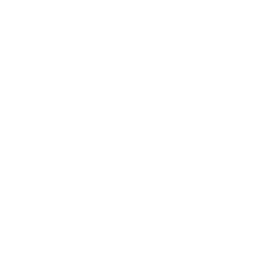
\includegraphics[scale=1]{assets/branding/opa0}
    \vspace{-5.75cm}\\
    {\adjustbox{scale=2.5}{\color{TealDarkCyan}\;I.\;Introduction}}
    \vspace{.25cm}
    \begin{minipage}{.78\textwidth}
      \scriptsize\color{Ink}
      \textbf{Big picture.}\; Lattice cryptography is a story about turning algebraic data into geometric search.\\[.2cm]
      \textbf{Details to watch.}\; basis, determinant, short vectors, dual tests, noise, and modular relations.
    \end{minipage}
    {\ }\vspace{2.1cm}\\
    \bigskip
  \end{center}
\end{frame}

\begin{frame}{\textbf{I. Introduction}}{Discrete Geometry}\small
\textcolor{TealDarkCyan}{\textbf{A lattice is a collection of periodic points.}}
\begin{itemize}
	\item It is discrete, but it fills all directions of a vector space.
	\item It has algebraic data: a basis and integer coefficients.
	\item It has geometric data: length, angle, volume, and distance.
\end{itemize}
\bigskip
\begin{center}
\begin{tikzpicture}[scale=.6]
\clip (-3.2,-2.6) rectangle (3.4,3.0);
\foreach \i in {-4,...,4}{
	\foreach \j in {-4,...,4}{
		\coordinate (p) at ({\i+0.42*\j},{0.72*\j});
		\node[lattice point] at (p) {};
	}
}
\draw[fill=AccentCyan!12,draw=AccentCyan!70,line width=.8pt]
(0,0) -- (1,0) -- (1.42,.72) -- (.42,.72) -- cycle;
\draw[basis vector, magenta] (0,0) -- (1,0) node[right] {$b_1$};
\draw[basis vector, magenta] (0,0) -- (.42,.72) node[above] {$b_2$};
\node[caption text,align=center] at (0,-1.25) {one basis\\ one fundamental cell};
\end{tikzpicture}
\end{center}
\bigskip
\textbf{\color{red}Question.}\; How hard is it to find the closest or shortest lattice vector?
\end{frame}

\begin{frame}{\textbf{I. Introduction}}{Build-up: From Lattices to Cryptography}
\small
\begin{columns}[T,onlytextwidth]
\begin{column}{.46\textwidth}
\textcolor{TealDarkCyan}{\textbf{Big picture}}
\begin{itemize}
  \item Lattices give a bridge from integer algebra to Euclidean geometry.
  \item Hard problems ask for hidden short or nearby structure.
  \item Cryptography publishes the algebra and hides the geometric witness.
\end{itemize}
\end{column}
\begin{column}{.50\textwidth}
\textcolor{TealDarkCyan}{\textbf{Details that will recur}}
\begin{itemize}
  \item \textbf{Shortness:} SIS and Module-SIS ask for short kernel relations.
  \item \textbf{Noise:} LWE, Ring-LWE, and Module-LWE blur exact equations.
  \item \textbf{Rounding:} LWR hides low-order information without sampled error.
\end{itemize}
\end{column}
\end{columns}
\begin{center}
\begin{tikzpicture}[node distance=.72cm,scale=.86,transform shape]
  \node[process] (basis) {basis\\$\mat B\Z^n$};
  \node[process blue,right=of basis] (geom) {geometry\\$\lambda_i,\det,\Ldual$};
  \node[process amber,right=of geom] (hard) {hard tasks\\SVP/CVP/SIS/LWE};
  \node[process red,right=of hard] (crypto) {crypto\\public algebra};
  \draw[flow] (basis) -- (geom);
  \draw[flow blue] (geom) -- (hard);
  \draw[flow amber] (hard) -- (crypto);
\end{tikzpicture}
\end{center}
\textbf{Teaching rule.}\; On each slide, separate the local calculation from the global question:
what public object is given, what hidden witness exists, and why finding it is hard.
\end{frame}

\begin{frame}{\textbf{I. Introduction}}{Why Lattices Matter: Geometry of Numbers}
\scriptsize
\begin{columns}[T,onlytextwidth]
\begin{column}{.60\textwidth}
\defbox[Q. What concrete problem does it solve?]{
\textbf{Example.}\;
In $\Z^2$, Minkowski's theorem says that any centrally symmetric convex region with area $>4$ contains a nonzero integer point.
The statement is geometric, but the conclusion is arithmetic: an integer solution must exist.

\textbf{What it reveals.}\;
A lattice point is not found by solving equations one-by-one; it is forced by volume.
For a general lattice, the threshold is $2^n\det(\Lat)$.

\textbf{Why important.}\;
This is the basic move of lattice theory: prove the existence of number-theoretic objects by showing that Euclidean space has no room to avoid them.}
\end{column}
\begin{column}{.36\textwidth}
\begin{center}
\begin{tikzpicture}[scale=.58]
  \draw[thin lattice line] (-2.6,-2.1) grid[step=.7] (2.6,2.1);
  \foreach \x in {-3,...,3}{
    \foreach \y in {-2,...,2}{
      \node[lattice point] at (.7*\x,.7*\y) {};
    }
  }
  \draw[fill=AccentCyan!13,draw=AccentCyan!80,line width=1pt]
    (0,0) ellipse (1.72 and 1.08);
  \node[circle,draw=ErrorRed,fill=ErrorRed!25,inner sep=2.2pt] at (.7,0) {};
  \node[tiny label,ErrorRed!85!black] at (1.45,.35) {forced point};
  \draw[flow red] (1.25,.25) -- (.75,.03);
  \node[caption text,align=center] at (0,-1.75)
    {$\vol(K)>4\det(\Z^2)$\\$\Rightarrow K\cap\Z^2\ne\{0\}$};
\end{tikzpicture}
\end{center}
\end{column}
\end{columns}
\end{frame}

\begin{frame}{\textbf{I. Introduction}}{Why Lattices Matter: Quadratic Forms}
\scriptsize
\begin{columns}[T,onlytextwidth]
\begin{column}{.58\textwidth}
\defbox[Q. What is the example?]{
\textbf{Example.}\;
The hexagonal lattice has basis
\[
  b_1=(1,0),\qquad b_2=(1/2,\sqrt{3}/2).
\]
For $z=(x,y)\in\Z^2$,
\[
  \norm{x b_1+y b_2}^2=x^2+xy+y^2.
\]

\textbf{What it reveals.}\;
The shortest nonzero vectors are exactly the integer solutions of
\[
  x^2+xy+y^2=1.
\]
There are six of them, which is why each disk in the hexagonal packing touches six neighbors.

\textbf{Why important.}\;
A quadratic form is not just algebraic notation; it is the length function of a lattice written in integer coordinates.}
\end{column}
\begin{column}{.38\textwidth}
\begin{center}
\begin{tikzpicture}[scale=.70]
  \clip (-2.15,-2.35) rectangle (2.25,2.05);
  \foreach \i in {-3,...,3}{
    \foreach \j in {-3,...,3}{
      \coordinate (p) at ({\i+.5*\j},{.866*\j});
      \node[lattice point] at (p) {};
    }
  }
  \draw[ErrorRed!35,line width=.8pt] (0,0) circle (1);
  \foreach \p in {(1,0),(-1,0),(.5,.866),(-.5,.866),(.5,-.866),(-.5,-.866)}{
    \draw[short vector] (0,0) -- \p;
  }
  \draw[basis vector] (0,0) -- (1,0) node[below] {$b_1$};
  \draw[basis vector] (0,0) -- (.5,.866) node[above right] {$b_2$};
  \node[tiny label,align=center,text width=3.0cm] at (0,-1.68)
    {$x^2+xy+y^2=1$\\six shortest vectors};
\end{tikzpicture}
\end{center}
\end{column}
\end{columns}
\end{frame}

\begin{frame}{\textbf{I. Introduction}}{Why Lattices Matter: Diophantine Approximation}
\scriptsize
\begin{columns}[T,onlytextwidth]
\begin{column}{.58\textwidth}
\defbox[Q. How does approximation become a lattice problem?]{
\textbf{Example.}\;
To approximate $\pi$, look for integers $p,q$ with $|p-q\pi|$ tiny.
The famous approximation
\[
  \frac{355}{113}\approx \pi
\]
means that the integer vector $(p,q)=(355,113)$ makes the linear form $p-q\pi$ unusually small.

\textbf{Lattice viewpoint.}\;
For a scale $N$, vectors of the form
\[
  (p-q\pi,\ q/N)
\]
balance two demands: small error and not-too-large denominator.

\textbf{Why important.}\;
Lattices explain why good approximations are short vectors: the numerator, denominator, and error become one geometric object.}
\end{column}
\begin{column}{.38\textwidth}
\begin{center}
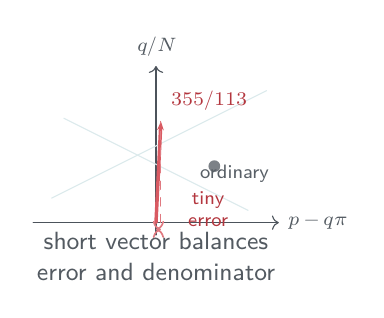
\begin{tikzpicture}[x=1cm,y=1cm,scale=.78]
  \draw[->,Ink!75] (-2.0,0) -- (2.0,0) node[right,tiny label] {$p-q\pi$};
  \draw[->,Ink!75] (0,-.2) -- (0,2.55) node[above,tiny label] {$q/N$};
  \draw[Grid,line width=.4pt] (-1.7,.4) -- (1.8,2.15);
  \draw[Grid,line width=.4pt] (-1.5,1.7) -- (1.5,.2);
  \node[circle,fill=Ink!55,inner sep=1.5pt] at (.95,.92) {};
  \node[tiny label,Ink!70] at (1.28,.8) {ordinary};
  \draw[short vector] (0,0) -- (.08,1.65)
    node[above right,tiny label,ErrorRed!85!black] {$355/113$};
  \draw[dashed,ErrorRed!70] (.08,0) -- (.08,1.65);
  \draw[<->,ErrorRed!70,line width=.6pt] (0,-.11) -- (.08,-.11);
  \node[tiny label,ErrorRed!85!black,align=center] at (.85,.22)
    {tiny\\error};
  \node[caption text,align=center] at (0,-.55)
    {short vector balances\\error and denominator};
\end{tikzpicture}
\end{center}
\end{column}
\end{columns}
\end{frame}

\begin{frame}{\textbf{I. Introduction}}{Why Lattices Matter: Sphere Packing}
\scriptsize
\begin{columns}[T,onlytextwidth]
\begin{column}{.56\textwidth}
\defbox[Q. What is the concrete packing example?]{
\textbf{Example.}\;
In the square lattice $\Z^2$, unit spacing gives disk density
\[
  \Delta(\Z^2)=\frac{\pi(1/2)^2}{1}=\frac{\pi}{4}\approx .785.
\]
In the hexagonal lattice, the same nearest-neighbor distance gives
\[
  \Delta=\frac{\pi}{\sqrt{12}}\approx .907.
\]

\textbf{What it reveals.}\;
The key quantities are the shortest vector length $\lambda_1(\Lat)$ and the cell area $\det(\Lat)$.

\textbf{Why important.}\;
The best two-dimensional packing is not discovered by drawing many circles; it is explained by the geometry of one lattice cell and its shortest vectors.}
\end{column}
\begin{column}{.40\textwidth}
\begin{center}
\begin{tikzpicture}[scale=.55]
  \begin{scope}[shift={(-2.0,0)}]
    \foreach \x in {-1,0,1}{
      \foreach \y in {-1,0,1}{
        \draw[fill=BlueCode!9,draw=BlueCode!35] (\x,\y) circle (.5);
        \node[lattice point] at (\x,\y) {};
      }
    }
    \draw[draw=BlueCode!80,line width=.8pt] (-.5,-.5) rectangle (.5,.5);
    \node[caption text,align=center] at (0,-1.85) {square\\$\pi/4$};
  \end{scope}
  \begin{scope}[shift={(2.25,0)}]
    \foreach \i in {-1,0,1}{
      \foreach \j in {-1,0,1}{
        \coordinate (p) at ({\i+.5*\j},{.866*\j});
        \draw[fill=AccentCyan!9,draw=AccentCyan!35] (p) circle (.5);
        \node[lattice point] at (p) {};
      }
    }
    \draw[draw=AccentCyan!85,line width=.8pt]
      (0,0) -- (1,0) -- (1.5,.866) -- (.5,.866) -- cycle;
    \node[caption text,align=center] at (.45,-1.85) {hexagonal\\$\pi/\sqrt{12}$};
  \end{scope}
  \node[caption text,align=center,text width=3.6cm] at (.18,2.0)
    {$\lambda_1$: disk radius\\$\det(\Lat)$: cell area};
\end{tikzpicture}
\end{center}
\end{column}
\end{columns}
\end{frame}

\begin{frame}{\textbf{I. Introduction}}{Why Lattices Matter: Integer Programming}
\scriptsize
\begin{columns}[T,onlytextwidth]
\begin{column}{.58\textwidth}
\defbox[Q. Where does lattice geometry enter optimization?]{
\textbf{Example.}\;
An integer program asks for a point in
\[
  P\cap\Z^n,
\]
where $P$ is a polytope. Its linear relaxation searches $P\cap\R^n$ instead.
A fractional optimum may sit near the middle of a face, while every nearby integer point violates a constraint.

\textbf{What it reveals.}\;
Rounding is a geometric question: how is the real feasible region positioned relative to the lattice $\Z^n$?
If $P$ is thin in some integer direction, that direction is the useful branch or cut.

\textbf{Why important.}\;
Lattice width, flatness, and rounding explain why continuous optimization is only the beginning of integer optimization.}
\end{column}
\begin{column}{.38\textwidth}
\begin{center}
\begin{tikzpicture}[scale=.66]
  \draw[thin lattice line] (-.4,-.4) grid[step=.65] (4.15,3.5);
  \foreach \x in {0,...,6}{
    \foreach \y in {0,...,5}{
      \node[circle,fill=Ink!55,inner sep=1.25pt] at (.65*\x,.65*\y) {};
    }
  }
  \draw[fill=AccentCyan!12,draw=AccentCyan!85,line width=1pt]
    (.42,.35) -- (3.65,.95) -- (2.25,2.72) -- (.72,2.05) -- cycle;
  \node[circle,fill=ErrorRed,inner sep=2.2pt] at (3.25,1.08) {};
  \node[tiny label,ErrorRed!85!black,align=center] at (3.12,1.48) {fractional\\optimum};
  \draw[flow red] (3.25,1.08) -- (2.6,1.3);
  \draw[ErrorRed!80,dashed,line width=.8pt] (.25,1.72) -- (3.9,2.4);
  \node[tiny label,ErrorRed!85!black,align=center] at (2.9,2.75) {cut / thin\\direction};
  \node[caption text,align=center,text width=3.45cm] at (1.8,-.8)
    {$P\cap\R^n$ is easy;\\$P\cap\Z^n$ depends on the grid};
\end{tikzpicture}
\end{center}
\end{column}
\end{columns}
\end{frame}

\begin{frame}{\textbf{I. Introduction}}{Why Lattices Matter: LLL Reduction}
\scriptsize
\begin{columns}[T,onlytextwidth]
\begin{column}{.58\textwidth}
\defbox[Q. What does LLL actually uncover?]{
\textbf{Example.}\;
The vectors
\[
  c_1=(1001,1000),\qquad c_2=(1000,999)
\]
form a basis of $\Z^2$ because $\det[c_1\ c_2]=-1$.
Both basis vectors have length about $1414$, but
\[
  c_1-c_2=(1,1)
\]
is very short.

\textbf{What it reveals.}\;
A basis can hide the geometry of its own lattice.
LLL performs integer column operations to expose shorter, more orthogonal directions.

\textbf{Why important.}\;
Many attacks and algorithms begin by asking: is the secret simply hidden by a bad basis? LLL is the first systematic test.}
\end{column}
\begin{column}{.38\textwidth}
\begin{center}
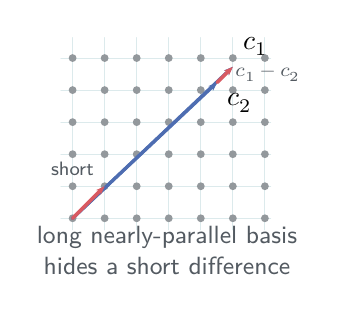
\begin{tikzpicture}[scale=.74]
  \draw[thin lattice line] (-.2,-.2) grid[step=.55] (3.4,3.1);
  \foreach \x in {0,...,6}{
    \foreach \y in {0,...,5}{
      \node[circle,fill=Ink!45,inner sep=1pt] at (.55*\x,.55*\y) {};
    }
  }
  \coordinate (O) at (0,0);
  \coordinate (cOne) at (2.75,2.6);
  \coordinate (cTwo) at (2.48,2.33);
  \draw[basis vector] (O) -- (cOne) node[above right] {$c_1$};
  \draw[basis vector] (O) -- (cTwo) node[below right] {$c_2$};
  \draw[short vector] (cTwo) -- (cOne) node[midway,right,tiny label] {$c_1-c_2$};
  \draw[short vector] (O) -- (.55,.55) node[above left,tiny label] {short};
  \node[caption text,align=center] at (1.62,-.55)
    {long nearly-parallel basis\\hides a short difference};
\end{tikzpicture}
\end{center}
\end{column}
\end{columns}
\end{frame}

\begin{frame}{\textbf{I. Introduction}}{Why Lattices Matter: Post-Quantum Cryptography}
\scriptsize
\begin{columns}[T,onlytextwidth]
\begin{column}{.58\textwidth}
\defbox[Q. What is the concrete cryptographic shape?]{
\textbf{Example.}\;
In LWE, the public data has the form
\[
  b=\mat A s+e\pmod q,
\]
where $s$ is secret and $e$ is small noise.
Without $e$, this is ordinary linear algebra modulo $q$.
With $e$, it becomes a noisy decoding problem.

\textbf{Lattice viewpoint.}\;
After lifting modulo $q$ to integers, $b$ is close to a structured $q$-ary lattice point, but the small error hides which one.

\textbf{Why important.}\;
Known quantum algorithms are excellent at exact algebraic structure; lattice cryptography deliberately adds controlled noise and shortness constraints.}
\end{column}
\begin{column}{.38\textwidth}
\begin{center}
\begin{tikzpicture}[scale=.64]
  \clip (-2.25,-2.15) rectangle (2.65,2.25);
  \foreach \i in {-3,...,3}{
    \foreach \j in {-3,...,3}{
      \coordinate (p) at ({\i+.45*\j},{.72*\j});
      \node[lattice point] at (p) {};
    }
  }
  \coordinate (As) at (.9,.72);
  \coordinate (b) at (1.18,.98);
  \draw[ErrorRed!35,fill=ErrorRed!7] (As) circle (.42);
  \node[circle,fill=BlueCode,inner sep=2pt,label={[tiny label]below:$\mat A s$}] at (As) {};
  \node[circle,fill=ErrorRed,inner sep=2pt] at (b) {};
  \node[tiny label,ErrorRed!85!black] at (1.55,1.12) {$b$};
  \draw[flow red] (As) -- node[midway,above,tiny label] {$e$} (b);
  \node[tiny label,align=center,text width=3.25cm,fill=white,inner sep=1.5pt] at (.1,-1.05)
    {without noise: linear algebra\\with noise: decoding};
\end{tikzpicture}
\end{center}
\end{column}
\end{columns}
\end{frame}

\begin{frame}{\textbf{I. Introduction}}{Why Lattices Matter: Worst-case to Average-case}
\scriptsize
\begin{columns}[T,onlytextwidth]
\begin{column}{.58\textwidth}
\defbox[Q. Why is this stronger than a random puzzle assumption?]{
\textbf{Example.}\;
A cryptographic public key should look random, so an attacker sees an average-case LWE or SIS instance, not a handcrafted worst-case lattice.

\textbf{Reduction idea.}\;
For suitable parameters, an algorithm that solves random LWE/SIS instances would imply algorithms for approximate GapSVP/SIVP on arbitrary lattices.
The random instance is tied back to the worst lattice geometry.

\textbf{Why important.}\;
This is rare in cryptography: the security evidence for random public instances is connected to broad worst-case mathematical hardness, not only to failed attack attempts.}
\end{column}
\begin{column}{.38\textwidth}
\begin{center}
\begin{tikzpicture}[node distance=.55cm,scale=.78,transform shape]
  \node[process red,minimum width=2.25cm] (worst) {arbitrary\\worst-case\\lattice};
  \node[process blue,below=of worst,minimum width=2.25cm] (reduce) {randomizing\\reduction};
  \node[process amber,below=of reduce,minimum width=2.25cm] (avg) {random\\LWE/SIS\\instance};
  \node[process,below=of avg,minimum width=2.25cm] (break) {average-case\\solver};
  \draw[flow red] (worst) -- (reduce);
  \draw[flow blue] (reduce) -- (avg);
  \draw[flow amber] (avg) -- (break);
  \draw[flow,bend left=42] (break.east) to node[right,tiny label,align=center] {would solve\\worst case} (worst.east);
\end{tikzpicture}
\end{center}
\end{column}
\end{columns}
\vfill
\textbf{Note.}\; The same object can be easy to describe by a basis and difficult to understand geometrically.
\end{frame}

\begin{frame}{\textbf{I. Introduction}}{The Dictionary}
\small
\begin{center}
\renewcommand{\arraystretch}{1.28}
\begin{tabular}{>{\bfseries}p{.28\textwidth}p{.62\textwidth}}
\toprule
Algebra & Geometry \\
\midrule
Basis matrix $\mat B$ & Skew coordinate grid in $\R^m$ \\
Integer vector $\vect z\in\Z^n$ & Lattice point $\mat B\vect z$ \\
Unimodular change $\mat U\in\GL_n(\Z)$ & Same lattice, different basis \\
$|\det \mat B|$ & Volume of a fundamental cell \\
Dual basis $\mat B^{-T}$ & Linear tests taking integer values \\
\bottomrule
\end{tabular}
\end{center}
\vfill
\textbf{\color{red}Warning.}\; A good coordinate system is not automatic. A bad basis can hide very short vectors.
\end{frame}

\begin{frame}{\textbf{I. Introduction}}{Roadmap}
\small
\begin{enumerate}
  \item Define lattices, bases, determinant, and the dual lattice.
  \item Use geometry of numbers to prove that short vectors must exist.
  \item State the main computational lattice problems.
  \item Explain why SIS, LWE, Ring-LWE, Module-LWE, LWR, and Module-SIS are lattice problems in disguise.
\end{enumerate}
\bigskip
\begin{center}
\begin{tikzpicture}[node distance=.7cm]
  \node[process] (basis) {basis};
  \node[process blue, right=1.1cm of basis] (geom) {geometry};
  \node[process amber, right=1.1cm of geom] (hard) {hard problems};
  \node[process red, right=1.1cm of hard] (crypto) {LWE/SIS\\families};
  \draw[flow] (basis) -- (geom);
  \draw[flow blue] (geom) -- (hard);
  \draw[flow amber] (hard) -- (crypto);
\end{tikzpicture}
\end{center}
\end{frame}


%-------------------------------------------------------
% II. LATTICES
%-------------------------------------------------------
\section{II. Lattices}
\HardProblemLens{A lattice basis is public algebra; the invariant object is a geometric point set with lengths and volume.}
%=======================================================
% CHAPTER 1: LATTICES
%=======================================================

\begin{frame}[plain]
  \begin{center}\bfseries\centering
    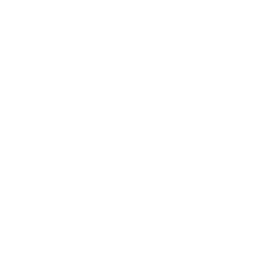
\includegraphics[scale=1]{assets/branding/opa0}
    \vspace{-5.75cm}\\
    {\adjustbox{scale=2.15}{\color{TealDarkCyan}\;II.\;Lattices}}
    \vspace{.25cm}
    \begin{minipage}{.78\textwidth}
      \scriptsize\color{Ink}
      \textbf{Big picture.}\; A basis is a coordinate description; the lattice is the invariant geometric object.\\[.2cm]
      \textbf{Details to watch.}\; integer combinations, basis changes, covolume, dual lattices, and Gram matrices.
    \end{minipage}
    {\ }\vspace{2.1cm}\\
    \bigskip
  \end{center}
\end{frame}

\begin{frame}[shrink=6]{\textbf{II. Lattices}}{Definition}
\defbox[Lattice generated by a basis]{
Let $b_1,\ldots,b_n\in\R^m$ be linearly independent. The lattice generated by them is
\[
  \Lat(\mat B)=\set{\sum_{i=1}^n z_i b_i : z_i\in\Z}
  = \mat B\Z^n,
\]
where $\mat B=[b_1\ \cdots\ b_n]\in\R^{m\times n}$.
}
\begin{itemize}
  \item The rank is $n$.
  \item The ambient dimension is $m$.
  \item A full-rank lattice in $\R^n$ has $m=n$.
\end{itemize}
\textbf{Equivalent viewpoint.}\; A lattice is a discrete additive subgroup of $\R^m$.

\textbf{Concrete example.}\; With $b_1=(2,0)$ and $b_2=(1,3)$,
\[
  \Lat=\set{u(2,0)+v(1,3):u,v\in\Z}
  =\set{(2u+v,3v):u,v\in\Z}.
\]
Thus $(4,6)=1b_1+2b_2\in\Lat$, while $(1,0)\notin\Lat$.
\end{frame}

\begin{frame}{\textbf{II. Lattices}}{Visualization: Integer Coordinates Become Geometry}
\small
\begin{center}
\begin{tikzpicture}[scale=.72]
  \begin{scope}[shift={(-4.1,-.55)}]
    \foreach \i in {-2,...,2}{
      \draw[thin lattice line] (\i,-2.2) -- (\i,2.2);
      \draw[thin lattice line] (-2.2,\i) -- (2.2,\i);
    }
    \foreach \i in {-2,...,2}{
      \foreach \j in {-2,...,2}{
        \node[lattice point] at (\i,\j) {};
      }
    }
    \draw[basis vector] (0,0) -- (1,0) node[below] {$e_1$};
    \draw[basis vector] (0,0) -- (0,1) node[left] {$e_2$};
    \node[circle,fill=ErrorRed,inner sep=2pt,label={[tiny label]above:$(2,1)$}] at (2,1) {};
    \node[caption text] at (0,-2.65) {coefficient lattice $\Z^2$};
  \end{scope}

  \node[process blue,align=center] (map) at (0,0.65)
    {$\mat B=\begin{bmatrix}2&1\\0&3\end{bmatrix}$\\[2pt]multiply by $\mat B$};
  \draw[flow blue] (-1.55,.55) -- (map.west);
  \draw[flow blue] (map.east) -- (1.55,.55);

  \begin{scope}[shift={(3.55,-.95)},scale=.46]
    \foreach \i in {-2,...,2}{
      \foreach \j in {-2,...,2}{
        \node[lattice point] at ({2*\i+\j},{3*\j}) {};
      }
    }
    \draw[basis vector] (0,0) -- (2,0) node[below] {$b_1=(2,0)$};
    \draw[basis vector] (0,0) -- (1,3) node[right] {$b_2=(1,3)$};
    \draw[short vector] (0,0) -- (5,3) node[above right] {$2b_1+b_2=(5,3)$};
    \node[circle,fill=ErrorRed,inner sep=2.5pt] at (5,3) {};
    \node[caption text,scale=1.15] at (1,-4.7) {$\mat B\Z^2$};
  \end{scope}
\end{tikzpicture}
\end{center}
\[
  (u,v)\in\Z^2\quad\longmapsto\quad u b_1+v b_2=(2u+v,3v).
\]
\textbf{Point.}\; A lattice basis is a linear machine that turns integer coordinates into a discrete geometric point set.
\end{frame}

\begin{frame}[shrink=8]{\textbf{II. Lattices}}{Many Bases, One Lattice}
\begin{columns}[T,onlytextwidth]
\begin{column}{.54\textwidth}
\thmbox[Change of basis]{
If $\mat B$ is a basis matrix and $\mat U\in\GL_n(\Z)$ is unimodular, then
\[
  \Lat(\mat B\mat U)=\Lat(\mat B).
\]
Conversely, two full-rank bases of the same lattice differ by such a matrix.
}
\begin{itemize}
  \item Unimodular means $\mat U$ has integer entries and determinant $\pm 1$.
  \item The lattice is the invariant object; the basis is only a coordinate choice.
\end{itemize}
\textbf{Example.}\; For $\mat U=\begin{bmatrix}1&1\\0&1\end{bmatrix}$,
\[
  [b_1\ b_2]\mat U=[b_1\ \ b_1+b_2].
\]
The basis changes, but the point set does not.
\end{column}
\begin{column}{.42\textwidth}
\begin{center}
\begin{tikzpicture}[scale=.62]
  \clip (-3.3,-2.5) rectangle (3.4,3.0);
  \foreach \i in {-4,...,4}{
    \foreach \j in {-4,...,4}{
      \node[lattice point] at ({\i+0.45*\j},{0.72*\j}) {};
    }
  }
  \draw[basis vector] (0,0) -- (1,0) node[below] {$b_1$};
  \draw[basis vector] (0,0) -- (.45,.72) node[right] {$b_2$};
  \draw[short vector] (0,0) -- (1.45,.72) node[above right] {$b'_1$};
  \draw[short vector] (0,0) -- (.45,.72) node[above left] {$b'_2$};
  \node[caption text,align=center] at (0,-2.0) {same points, different bases};
\end{tikzpicture}
\end{center}
\end{column}
\end{columns}
\end{frame}

\begin{frame}[shrink=5]{\textbf{II. Lattices}}{Fundamental Parallelepiped}
\defbox[Fundamental parallelepiped]{
For a basis $\mat B=[b_1\ \cdots\ b_n]$ of a full-rank lattice,
\[
  \fund(\mat B)=\set{\sum_{i=1}^n t_i b_i : 0\le t_i<1}.
\]
Every $x\in\R^n$ has a unique decomposition $x=v+p$ with $v\in\Lat$ and $p\in\fund(\mat B)$.
}
\begin{columns}[T,onlytextwidth]
\begin{column}{.45\textwidth}
\begin{itemize}
  \item $\fund(\mat B)$ tiles the space by lattice translations.
  \item It is a coordinate-dependent fundamental domain.
\end{itemize}
\textbf{Example in $\Z^2$.}\; For $\mat B=\mat I_2$,
\[
  (2.7,-1.3)=(2,-2)+(0.7,0.7).
\]
The first term is in $\Z^2$; the second lies in $[0,1)^2$.
\end{column}
\begin{column}{.50\textwidth}
\begin{center}
\begin{tikzpicture}[scale=.58]
  \clip (-3.1,-1.8) rectangle (3.7,3.0);
  \foreach \i in {-3,...,3}{
    \foreach \j in {-3,...,3}{
      \draw[thin lattice line] ({\i+0.5*\j},{.8*\j}) -- ({\i+1+0.5*\j},{.8*\j});
      \draw[thin lattice line] ({\i+0.5*\j},{.8*\j}) -- ({\i+0.5*(\j+1)},{.8*(\j+1)});
      \node[lattice point] at ({\i+0.5*\j},{.8*\j}) {};
    }
  }
  \draw[fill=AccentCyan!18,draw=AccentCyan!80,line width=1pt]
    (0,0) -- (1,0) -- (1.5,.8) -- (.5,.8) -- cycle;
  \node[caption text] at (1,.38) {$\fund(\mat B)$};
\end{tikzpicture}
\end{center}
\end{column}
\end{columns}
\end{frame}

\begin{frame}{\textbf{II. Lattices}}{Determinant and Covolume}
\scriptsize
\defbox[Determinant]{
For a full-rank lattice $\Lat=\Lat(\mat B)\subset\R^n$,
\[
  \det(\Lat)=|\det \mat B|.
\]
Equivalently, $\det(\Lat)$ is the volume of any fundamental parallelepiped.
}
\begin{itemize}
  \item This number is independent of the basis:
  \[
    |\det(\mat B\mat U)|=|\det \mat B|\,|\det \mat U|=|\det \mat B|.
  \]
  \item Small determinant means many lattice points per unit volume; large determinant means sparse lattice points.
\end{itemize}
\vspace{-.2cm}
\probox[Counting heuristic]{
For a reasonably round region $S\subset\R^n$,
\[
  |\Lat\cap S| \approx \frac{\vol(S)}{\det(\Lat)}.
\]
}
\textbf{Example.}\; If $b_1=(2,0)$ and $b_2=(1,3)$, then $\det(\Lat)=6$.
A region of area $600$ should contain roughly $600/6=100$ lattice points.
\end{frame}

\begin{frame}{\textbf{II. Lattices}}{Visualization: Covolume Measures Density}
\small
\begin{columns}[T,onlytextwidth]
\begin{column}{.58\textwidth}
\begin{center}
\begin{tikzpicture}[scale=.55]
  \begin{scope}[shift={(-2.8,0)}]
    \draw[panel] (-2.25,-1.85) rectangle (2.25,2.15);
    \foreach \i in {-3,...,3}{
      \foreach \j in {-3,...,3}{
        \node[lattice point] at ({.72*\i+.25*\j},{.65*\j}) {};
      }
    }
    \draw[fill=TealDarkCyan!12,draw=TealDarkCyan,line width=.9pt]
      (0,0) -- (.72,0) -- (.97,.65) -- (.25,.65) -- cycle;
    \node[caption text,align=center] at (0,-2.35) {small cell\\many points};
  \end{scope}
  \begin{scope}[shift={(2.8,0)}]
    \draw[panel] (-2.25,-1.85) rectangle (2.25,2.15);
    \foreach \i in {-2,...,2}{
      \foreach \j in {-2,...,2}{
        \node[lattice point] at ({1.35*\i+.55*\j},{1.10*\j}) {};
      }
    }
    \draw[fill=AmberCode!14,draw=AmberCode,line width=.9pt]
      (0,0) -- (1.35,0) -- (1.90,1.10) -- (.55,1.10) -- cycle;
    \node[caption text,align=center] at (0,-2.35) {large cell\\few points};
  \end{scope}
\end{tikzpicture}
\end{center}
\end{column}
\begin{column}{.38\textwidth}
\textbf{Same window, different covolume.}
\[
  \#(\Lat\cap S)\approx \frac{\vol(S)}{\det(\Lat)}.
\]
\textbf{Concrete reading.}\; If the fundamental cell has area $6$, then each lattice point occupies about six square units of plane.
\end{column}
\end{columns}
\end{frame}

\begin{frame}[shrink=5]{\textbf{II. Lattices}}{The Dual Lattice}
\defbox[Dual lattice]{
The dual lattice is
\[
  \Ldual=\set{y\in\Span(\Lat):\inner{x}{y}\in\Z\ \text{for all }x\in\Lat}.
\]
If $\Lat=\Lat(\mat B)$ is full-rank, then
\[
  \Ldual=\Lat(\mat B^{-T}).
\]
}
\begin{columns}[T,onlytextwidth]
\begin{column}{.48\textwidth}
\textcolor{TealDarkCyan}{\textbf{Facts}}
\begin{itemize}
  \item $(\Ldual)^{*}=\Lat$.
  \item $\det(\Ldual)=1/\det(\Lat)$.
  \item Dual vectors define integer-valued tests on $\Lat$.
\end{itemize}
\end{column}
\begin{column}{.48\textwidth}
\textcolor{TealDarkCyan}{\textbf{Cryptographic role}}
\begin{itemize}
  \item Modular equations define $q$-ary lattices.
  \item Fourier analysis naturally sees the dual lattice.
  \item LWE noise is measured relative to dual constraints.
\end{itemize}
\end{column}
\end{columns}
\textbf{Concrete test.}\; If $\Lat=2\Z\times 3\Z$, then $\Ldual=\frac12\Z\times\frac13\Z$.
The vector $y=(1/2,1/3)$ is dual because
$\inner{(2a,3b)}{y}=a+b\in\Z$.
\end{frame}

\begin{frame}{\textbf{II. Lattices}}{Visualization: Dual Vectors Are Integer Tests}
\small
\begin{columns}[T,onlytextwidth]
\begin{column}{.50\textwidth}
\begin{center}
\begin{tikzpicture}[scale=.64,transform shape]
  \useasboundingbox (-3.0,-2.55) rectangle (3.0,2.2);
  \begin{scope}[rotate=-34]
    \foreach \k in {-3,...,3}{
      \draw[BlueCode!24,line width=.6pt] (-3.0,{.56*\k}) -- (3.0,{.56*\k});
    }
  \end{scope}
  \foreach \i in {-2,...,2}{
    \foreach \j in {-2,...,2}{
      \node[lattice point] at ({.95*\i+.38*\j},{.63*\j}) {};
    }
  }
  \draw[short vector] (0,0) -- (.92,.62) node[right] {$y\in\Ldual$};
  \node[tiny label,fill=white,inner sep=1pt] at (-2.45,1.65) {$\inner{x}{y}=-1$};
  \node[tiny label,fill=white,inner sep=1pt] at (-1.25,.55) {$\inner{x}{y}=0$};
  \node[tiny label,fill=white,inner sep=1pt] at (.25,-.55) {$\inner{x}{y}=1$};
  \node[caption text,align=center,text width=5.1cm] at (0,-2.10)
    {level sets of the test $x\mapsto\inner{x}{y}$};
\end{tikzpicture}
\end{center}
\end{column}
\begin{column}{.46\textwidth}
\textbf{Interpretation.}\; A dual vector does not merely point in space. It defines a ruler:
\[
  x\in\Lat\quad\Longrightarrow\quad \inner{x}{y}\in\Z.
\]
\textbf{Concrete example.}\; For $\Lat=2\Z\times3\Z$, the dual vector
$y=(1/2,1/3)$ sends $(2a,3b)$ to $a+b$.
\end{column}
\end{columns}
\end{frame}

\begin{frame}[shrink=8]{\textbf{II. Lattices}}{Gram Matrix}
\defbox[Gram matrix]{
Given a basis $\mat B=[b_1\ \cdots\ b_n]$, the Gram matrix is
\[
  \mat G=\mat B^T\mat B,\qquad G_{ij}=\inner{b_i}{b_j}.
\]
}
\begin{itemize}
  \item $\mat G$ stores all lengths and angles of the basis vectors.
  \item $\det(\mat G)=(\det\mat B)^2$ for full-rank square $\mat B$.
  \item Quadratic forms appear because
  \[
    \norm{\mat B z}^2=z^T\mat G z,\qquad z\in\Z^n.
  \]
\end{itemize}
\bigskip
\thmbox[Key reduction]{
Finding a short nonzero lattice vector is equivalent to minimizing a positive definite quadratic form over $\Z^n\setdiff\{0\}$.
}
\textbf{Example.}\; For $b_1=(2,0)$ and $b_2=(1,3)$,
\[
  \mat G=\begin{bmatrix}4&2\\2&10\end{bmatrix},\qquad
  \norm{x b_1+y b_2}^2=4x^2+4xy+10y^2.
\]
\end{frame}

\begin{frame}{\textbf{II. Lattices}}{Visualization: The Gram Matrix Stores Angles}
\small
\begin{columns}[T,onlytextwidth]
\begin{column}{.48\textwidth}
\begin{center}
\begin{tikzpicture}[scale=.82]
  \coordinate (O) at (0,0);
  \coordinate (B1) at (3.1,0);
  \coordinate (B2) at (1.25,2.15);
  \coordinate (P) at (1.25,0);
  \draw[fill=TealDarkCyan!10,draw=TealDarkCyan!40] (O) -- (B1) -- ($(B1)+(B2)$) -- (B2) -- cycle;
  \draw[basis vector] (O) -- (B1) node[below] {$b_1$};
  \draw[basis vector] (O) -- (B2) node[left] {$b_2$};
  \draw[ErrorRed!70,dashed] (B2) -- (P);
  \draw[ErrorRed!70,dashed] (P) -- (O);
  \pic[draw=AmberCode,fill=AmberCode!12,angle radius=.62cm,"$\theta$"{font=\scriptsize}] {angle=B1--O--B2};
  \node[tiny label] at (1.55,-.28) {projection};
  \node[caption text] at (1.7,2.85) {area$^2=\det(\mat G)$};
\end{tikzpicture}
\end{center}
\end{column}
\begin{column}{.48\textwidth}
\[
  \mat G=
  \begin{bmatrix}
  \norm{b_1}^2 & \inner{b_1}{b_2}\\
  \inner{b_2}{b_1} & \norm{b_2}^2
  \end{bmatrix}.
\]
\textbf{Why it matters.}\; Minimizing $\norm{\mat Bz}$ is the same as minimizing
\[
  z^T\mat Gz.
\]
So geometry becomes arithmetic in a positive definite quadratic form.
\end{column}
\end{columns}
\end{frame}


%-------------------------------------------------------
% III. GEOMETRY OF NUMBERS
%-------------------------------------------------------
\section{III. Geometry of Numbers}
\HardProblemLens{Volume arguments prove short structure exists, while algorithms still have to find it.}
%=======================================================
% CHAPTER 2: GEOMETRY OF NUMBERS
%=======================================================

\begin{frame}[plain]
  \begin{center}\bfseries\centering
    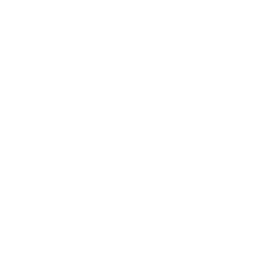
\includegraphics[scale=1]{assets/branding/opa0}
    \vspace{-5.75cm}\\
    {\adjustbox{scale=1.75}{\color{TealDarkCyan}\;III.\;Geometry of Numbers}}
    \vspace{.25cm}
    \begin{minipage}{.78\textwidth}
      \scriptsize\color{Ink}
      \textbf{Big picture.}\; Geometry proves that short structure must exist before algorithms try to find it.\\[.2cm]
      \textbf{Details to watch.}\; successive minima, Minkowski bounds, Gaussian heuristic, and packing density.
    \end{minipage}
    {\ }\vspace{2.1cm}\\
    \bigskip
  \end{center}
\end{frame}

\begin{frame}[shrink=5]{\textbf{III. Geometry of Numbers}}{Shortest Vector}
\defbox[First minimum]{
The first successive minimum of $\Lat$ is
\[
  \lambda_1(\Lat)=\min\set{\norm{v}:v\in\Lat\setdiff\{0\}}.
\]
Any nonzero $v\in\Lat$ with $\norm v=\lambda_1(\Lat)$ is a shortest vector.
}
\begin{columns}[T,onlytextwidth]
\begin{column}{.52\textwidth}
\begin{itemize}
  \item $\lambda_1$ is geometric: it does not depend on the basis.
  \item It is hard to read from a badly skewed basis.
  \item Cryptography uses the gap between basis description and geometric search.
\end{itemize}
\textbf{Example.}\; For $\Lat=2\Z\times5\Z$, the shortest nonzero vectors are $(\pm2,0)$, so $\lambda_1(\Lat)=2$.
\end{column}
\begin{column}{.43\textwidth}
\begin{center}
\begin{tikzpicture}[scale=.62]
  \clip (-3.3,-2.5) rectangle (3.3,2.7);
  \foreach \i in {-4,...,4}{
    \foreach \j in {-4,...,4}{
      \node[lattice point] at ({\i+0.38*\j},{0.72*\j}) {};
    }
  }
  \draw[short vector] (0,0) -- (1,0) node[below] {$\lambda_1$};
  \draw[basis vector] (0,0) -- (.38,.72) node[above left] {$b_2$};
  \draw[basis vector] (0,0) -- (2.14,.72) node[above right] {$b_1$};
  \draw[ErrorRed!35,line width=.9pt] (0,0) circle (1);
  \node[caption text] at (0,-2.05) {shortest vector versus basis vectors};
\end{tikzpicture}
\end{center}
\end{column}
\end{columns}
\end{frame}

\begin{frame}[shrink=8]{\textbf{III. Geometry of Numbers}}{Successive Minima}
\defbox[Successive minima]{
For $1\le i\le n$, the $i$-th successive minimum is
\[
  \lambda_i(\Lat)
  =\inf\set{r>0:\dim\Span(\Lat\cap r\ball_2^n)\ge i}.
\]
}
\begin{itemize}
  \item $\lambda_i$ is the radius needed to find $i$ linearly independent lattice vectors.
  \item The sequence is monotone:
  \[
    \lambda_1(\Lat)\le \lambda_2(\Lat)\le \cdots\le \lambda_n(\Lat).
  \]
  \item The last minimum $\lambda_n$ measures how large a ball must be to reveal a full-rank lattice basis.
\end{itemize}
\vspace{-.15cm}
\textbf{Example.}\; For $\Lat=2\Z\times5\Z\subset\R^2$,
\[
  \lambda_1(\Lat)=2,\qquad \lambda_2(\Lat)=5.
\]
Radius $2$ finds one direction; radius $5$ finds two independent directions.
\vspace{-.15cm}
\begin{center}
\begin{tikzpicture}[scale=.58]
  \draw[ErrorRed!30,line width=.7pt] (0,0) circle (.8);
  \draw[BlueCode!30,line width=.7pt] (0,0) circle (1.45);
  \draw[GoodGreen!45!black,line width=.7pt] (0,0) circle (2.1);
  \node[lattice point] at (0,0) {};
  \node[lattice point] at (.8,0) {};
  \node[lattice point] at (-.8,0) {};
  \node[lattice point] at (.55,1.34) {};
  \node[lattice point] at (-.55,-1.34) {};
  \node[lattice point] at (1.35,1.34) {};
  \node[tiny label,ErrorRed!80!black] at (.58,.47) {$\lambda_1$};
  \node[tiny label,BlueCode!80!black] at (1.22,.9) {$\lambda_2$};
\end{tikzpicture}
\end{center}
\end{frame}

\begin{frame}[shrink=5]{\textbf{III. Geometry of Numbers}}{Minkowski's Convex Body Theorem}
\thmbox[Minkowski]{
Let $\Lat\subset\R^n$ be a full-rank lattice and let $K\subset\R^n$ be convex, centrally symmetric, and measurable. If
\[
  \vol(K)>2^n\det(\Lat),
\]
then $K$ contains a nonzero lattice point.
}
\begin{columns}[T,onlytextwidth]
\begin{column}{.47\textwidth}
\textcolor{TealDarkCyan}{\textbf{Meaning}}
\begin{itemize}
  \item Large symmetric bodies cannot avoid all nonzero lattice points.
  \item Volume alone forces arithmetic structure.
\end{itemize}
\end{column}
\begin{column}{.49\textwidth}
\textcolor{TealDarkCyan}{\textbf{Why the factor $2^n$?}}
\begin{itemize}
  \item Compare $K/2$ with a fundamental domain.
  \item If two points of $K/2$ are congruent modulo $\Lat$, their difference lies in $K\cap\Lat$.
\end{itemize}
\end{column}
\end{columns}
\textbf{Example in $\Z^2$.}\; Any centrally symmetric convex region with area $>4$ contains a nonzero integer point.
A long thin diamond can force an integer relation even when no coordinate is individually small.
\end{frame}

\begin{frame}[shrink=8]{\textbf{III. Geometry of Numbers}}{A Short Vector Always Exists}
\corbox[Minkowski bound for $\lambda_1$]{
For every full-rank lattice $\Lat\subset\R^n$,
\[
  \lambda_1(\Lat)\le \sqrt{n}\,\det(\Lat)^{1/n}.
\]
}
\textbf{Proof idea.}
\begin{itemize}
  \item Apply Minkowski's theorem to a cube centered at the origin.
  \item Choose side length slightly larger than $2\det(\Lat)^{1/n}$.
  \item The cube contains a nonzero lattice point $v$ with
  \[
    \norm v_2\le \sqrt{n}\,\det(\Lat)^{1/n}.
  \]
\end{itemize}
\bigskip
\textbf{\color{red}Important.}\; Existence is not an efficient algorithm for finding such a vector.
\textbf{Example.}\; In dimension $2$, if $\det(\Lat)=25$, Minkowski gives
\[
  \lambda_1(\Lat)\le \sqrt2\cdot5\approx 7.07.
\]
So a nonzero vector of length at most $7.07$ must exist, even if the displayed basis is much longer.
\end{frame}

\begin{frame}[shrink=8]{\textbf{III. Geometry of Numbers}}{Gaussian Heuristic}
\probox[Heuristic estimate]{
The expected number of lattice points in a ball of radius $r$ is approximately
\[
  \frac{\vol(r\ball_2^n)}{\det(\Lat)}.
\]
The Gaussian heuristic predicts $\lambda_1(\Lat)$ by setting this ratio near $1$.
}
\[
  \vol(r\ball_2^n)=
  \frac{\pi^{n/2}}{\Gamma(n/2+1)}r^n.
\]
\begin{itemize}
  \item Random-looking lattices often behave close to this estimate.
  \item Cryptographic parameter choices compare attacks against this geometry.
  \item The heuristic is not a theorem for every lattice.
\end{itemize}
\textbf{Example.}\; In $\R^2$ with $\det(\Lat)=100$, the heuristic expects one lattice point in a disk when
\[
  \pi r^2/100\approx1,\qquad r\approx\sqrt{100/\pi}\approx5.64.
\]
This is a prediction, not a guarantee.
\end{frame}

\begin{frame}[shrink=5]{\textbf{III. Geometry of Numbers}}{Sphere Packing Viewpoint}
Place a ball of radius $\lambda_1(\Lat)/2$ around each lattice point. These balls do not overlap.
\begin{center}
\begin{tikzpicture}[scale=.56]
  \clip (-3.3,-2.6) rectangle (3.5,2.9);
  \foreach \i in {-4,...,4}{
    \foreach \j in {-4,...,4}{
      \coordinate (p) at ({\i+0.45*\j},{0.78*\j});
      \draw[AccentCyan!20,fill=AccentCyan!7] (p) circle (.38);
      \node[lattice point] at (p) {};
    }
  }
  \draw[short vector] (0,0) -- (1,0) node[midway,below] {$\lambda_1$};
  \node[caption text] at (0,-2.25) {lattice packing by equal balls};
\end{tikzpicture}
\end{center}
\[
  \Delta(\Lat)=\frac{\vol((\lambda_1(\Lat)/2)\ball_2^n)}{\det(\Lat)}
\]
is the density of the corresponding lattice sphere packing.
\textbf{Example.}\; For $\Z^2$, $\lambda_1=1$ and $\det=1$, so the packing density is
$\pi(1/2)^2=\pi/4$.
Changing the lattice shape to the hexagonal lattice improves the density.
\end{frame}

\begin{frame}[shrink=8]{\textbf{III. Geometry of Numbers}}{Hermite Constant}
\defbox[Hermite invariant]{
For a full-rank lattice $\Lat\subset\R^n$,
\[
  \gamma(\Lat)=\frac{\lambda_1(\Lat)^2}{\det(\Lat)^{2/n}}.
\]
The Hermite constant is
\[
  \gamma_n=\sup_{\Lat\subset\R^n}\gamma(\Lat).
\]
}
\begin{itemize}
  \item It asks for the densest possible short-vector behavior in dimension $n$.
  \item It is closely tied to optimal lattice sphere packings.
  \item Computational lattice reduction is, in part, an attempt to find bases witnessing small vectors.
\end{itemize}
\textbf{Dimension $2$.}\; The square lattice has $\gamma(\Z^2)=1$.
The hexagonal lattice has $\lambda_1=1$ and $\det=\sqrt3/2$, hence
\[
  \gamma=\frac{1}{\sqrt3/2}=\frac{2}{\sqrt3}=\gamma_2.
\]
It is optimal in the plane.
\end{frame}


%-------------------------------------------------------
% IV. HARD PROBLEMS
%-------------------------------------------------------
\section{IV. Hard Problems}
\HardProblemLens{SVP, CVP, SIVP, and GapSVP isolate the search and decision tasks that reductions rely on.}
%=======================================================
% CHAPTER 3: HARD PROBLEMS
%=======================================================

\begin{frame}[plain]
  \begin{center}\bfseries\centering
    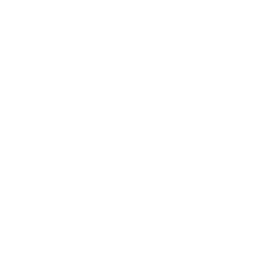
\includegraphics[scale=1]{assets/branding/opa0}
    \vspace{-5.75cm}\\
    {\adjustbox{scale=1.95}{\color{TealDarkCyan}\;IV.\;Hard Problems}}
    \vspace{.25cm}
    \begin{minipage}{.78\textwidth}
      \scriptsize\color{Ink}
      \textbf{Big picture.}\; Hardness comes from the gap between an easy basis description and hard geometric search.\\[.2cm]
      \textbf{Details to watch.}\; SVP, CVP, BDD, SIVP, GapSVP, LLL, and approximation factors.
    \end{minipage}
    {\ }\vspace{2.1cm}\\
    \bigskip
  \end{center}
\end{frame}

\begin{frame}[shrink=5]{\textbf{IV. Hard Problems}}{SVP}
\defbox[Shortest Vector Problem]{
Given a basis $\mat B$ of a lattice $\Lat$, find a nonzero vector $v\in\Lat$ such that
\[
  \norm v=\lambda_1(\Lat).
\]
}
\begin{columns}[T,onlytextwidth]
\begin{column}{.50\textwidth}
\textcolor{TealDarkCyan}{\textbf{Approximate SVP}}
\[
  \norm v\le \gamma(n)\lambda_1(\Lat).
\]
\begin{itemize}
  \item Exact SVP is too strong for many applications.
  \item Approximation factors encode the security target.
\end{itemize}
\end{column}
\begin{column}{.46\textwidth}
\textcolor{TealDarkCyan}{\textbf{Basis trap}}
\begin{itemize}
  \item A basis vector may be exponentially longer than $\lambda_1$.
  \item Short combinations can have large integer coefficients in a bad basis.
\end{itemize}
\end{column}
\end{columns}
\textbf{Toy instance.}\; For $\Lat=2\Z\times5\Z$, SVP returns $(\pm2,0)$ and $\lambda_1=2$.
With $c_1=(1001,1000)$, $c_2=(1000,999)$, the short vector is hidden as $c_1-c_2=(1,1)$.
\end{frame}

\begin{frame}[shrink=5]{\textbf{IV. Hard Problems}}{CVP}
\defbox[Closest Vector Problem]{
Given a basis of $\Lat\subset\R^n$ and a target $t\in\R^n$, find $v\in\Lat$ minimizing
\[
  \norm{t-v}.
\]
}
\begin{columns}[T,onlytextwidth]
\begin{column}{.52\textwidth}
\begin{itemize}
  \item CVP asks for the lattice point in the same Voronoi cell as $t$.
  \item Bounded Distance Decoding (BDD) is CVP with a promise that $t$ is close to the lattice.
  \item Decoding linear codes and decoding lattices are parallel ideas.
\end{itemize}
\textbf{Example in $\Z^2$.}\; For $t=(2.2,4.7)$, the closest point is $(2,5)$.
For a skew lattice, nearest-point search is no longer coordinate-wise rounding.
\end{column}
\begin{column}{.43\textwidth}
\begin{center}
\begin{tikzpicture}[scale=.62]
  \clip (-3,-2.6) rectangle (3.3,2.8);
  \foreach \i in {-4,...,4}{
    \foreach \j in {-4,...,4}{
      \node[lattice point] at ({\i+0.48*\j},{0.78*\j}) {};
    }
  }
  \coordinate (t) at (1.22,.52);
  \node[circle,fill=ErrorRed,inner sep=2pt,label=right:$t$] at (t) {};
  \draw[flow red] (t) -- (1,0) node[midway,right,tiny label] {error};
  \draw[ErrorRed!35,line width=.8pt] (1,0) circle (.78);
  \node[caption text] at (0,-2.15) {closest lattice point to a target};
\end{tikzpicture}
\end{center}
\end{column}
\end{columns}
\end{frame}

\begin{frame}[shrink=8]{\textbf{IV. Hard Problems}}{SIVP and GapSVP}
\begin{columns}[T,onlytextwidth]
\begin{column}{.48\textwidth}
\defbox[SIVP]{
Given a basis of $\Lat$, find $n$ linearly independent vectors
\[
  v_1,\ldots,v_n\in\Lat
\]
with $\max_i\norm{v_i}\le \gamma(n)\lambda_n(\Lat)$.
}
\end{column}
\begin{column}{.48\textwidth}
\defbox[GapSVP]{
Given a threshold $d$, distinguish between
\[
  \lambda_1(\Lat)\le d
  \quad\text{and}\quad
  \lambda_1(\Lat)>\gamma(n)d.
\]
}
\end{column}
\end{columns}
\bigskip
\textcolor{TealDarkCyan}{\textbf{Why they appear in reductions}}
\begin{itemize}
  \item SIVP captures the need for many independent short directions.
  \item GapSVP turns search geometry into a decision problem.
  \item Worst-case reductions often target approximate versions of these problems.
\end{itemize}
\textbf{Example.}\; For $\Lat=2\Z\times5\Z$, SIVP needs $(2,0)$ and $(0,5)$.
GapSVP with $d=3$ and $\gamma=2$ asks whether $\lambda_1\le3$ or $\lambda_1>6$.
\end{frame}

\begin{frame}[shrink=5]{\textbf{IV. Hard Problems}}{Naive Algorithms}
\textcolor{TealDarkCyan}{\textbf{Enumeration}}
\begin{itemize}
  \item Search all integer vectors $z$ with $\norm{\mat Bz}\le R$.
  \item Works in low dimensions.
  \item The search tree grows exponentially with the dimension.
\end{itemize}
\bigskip
\textcolor{TealDarkCyan}{\textbf{Voronoi methods}}
\begin{itemize}
  \item Describe the Voronoi cell and use its facets.
  \item Exact but exponential.
\end{itemize}
\bigskip
\textbf{\color{red}Lesson.}\; Exact lattice problems are feasible for small $n$ and become rapidly expensive.
\textbf{Enumeration scale.}\; If $z_i\in[-10,10]$, brute force checks $21^n$ candidates:
$441$ in dimension $2$, but about $1.7\times10^{13}$ in dimension $10$.
\end{frame}

\begin{frame}{\textbf{IV. Hard Problems}}{Visualization: Enumeration Explosion}
\small
\begin{columns}[T,onlytextwidth]
\begin{column}{.43\textwidth}
\textbf{Coefficient search.}\; Enumeration searches integer coordinates first:
\[
  z=(z_1,\ldots,z_n),\qquad \norm{\mat Bz}\le R.
\]
If each coordinate has $2R+1$ choices, the raw search width is
\[
  (2R+1)^n.
\]
\textbf{The geometry filters candidates, but the tree is still exponential.}
\end{column}
\begin{column}{.53\textwidth}
\begin{center}
\begin{tikzpicture}[scale=.72]
  \node[process] (root) at (0,1.8) {$z_1$};
  \foreach \x/\lab [count=\k] in {-2/-1,0/0,2/1}{
    \node[process blue,minimum width=.8cm] (a\k) at (\x,.65) {$\lab$};
    \draw[flow] (root) -- (a\k);
    \foreach \d/\labtwo in {-.55/-1,0/0,.55/1}{
      \node[circle,draw=AmberCode!65,fill=AmberCode!10,inner sep=2.0pt] at ({\x+\d},-.55) {};
      \draw[flow amber] (a\k) -- ({\x+\d},-.55);
    }
  }
  \node[tiny label] at (-2.55,-.95) {$z_2=-1,0,1$};
  \node[tiny label] at (0,-1.35) {$3^2$ partial nodes};
  \node[process red,align=center] at (0,-2.25)
    {after $n$ levels:\\$(2R+1)^n$ candidates};
\end{tikzpicture}
\end{center}
\end{column}
\end{columns}
\end{frame}

\begin{frame}[shrink=8]{\textbf{IV. Hard Problems}}{LLL Reduction}
\defbox[Goal of basis reduction]{
Replace a bad basis by a better basis of the same lattice:
\[
  \mat B\longmapsto \mat B\mat U,\qquad \mat U\in\GL_n(\Z).
\]
}
\thmbox[LLL theorem, informal]{
The LLL algorithm runs in polynomial time and outputs a basis whose first vector satisfies
\[
  \norm{b_1}\le 2^{(n-1)/2}\lambda_1(\Lat).
\]
}
\begin{itemize}
  \item LLL is powerful in practice but gives an exponential approximation factor.
  \item Stronger block reduction algorithms trade more time for better quality.
  \item Lattice cryptography chooses parameters beyond known reduction attacks.
\end{itemize}
\textbf{Concrete effect.}\; Starting from $c_1=(1001,1000)$ and $c_2=(1000,999)$, integer subtraction exposes
\[
  c_1-c_2=(1,1).
\]
LLL automates this kind of basis improvement in high dimension.
\end{frame}

\begin{frame}{\textbf{IV. Hard Problems}}{Visualization: LLL Finds Integer Cancellations}
\small
\begin{columns}[T,onlytextwidth]
\begin{column}{.51\textwidth}
\begin{center}
\begin{tikzpicture}[scale=.68,transform shape]
  \useasboundingbox (-.45,-2.75) rectangle (3.85,2.65);
  \coordinate (O) at (0,0);
  \coordinate (C1) at (3.35,2.25);
  \coordinate (C2) at (3.05,1.95);
  \draw[basis vector] (O) -- (C1) node[above] {$c_1$};
  \draw[basis vector] (O) -- (C2) node[below right] {$c_2$};
  \draw[short vector] (C2) -- (C1) node[midway,right] {$c_1-c_2$};
  \draw[TealDarkCyan!35,dashed] (2.65,1.55) rectangle (3.65,2.55);
  \begin{scope}[shift={(.35,-1.55)},scale=1.35]
    \draw[panel] (-.25,-.25) rectangle (1.25,1.25);
    \draw[short vector] (0,0) -- (1,1) node[above right] {$(1,1)$};
    \node[tiny label] at (.55,-.18) {zoom};
  \end{scope}
  \node[caption text,align=center,text width=4.2cm] at (1.7,-2.45)
    {a very short vector can be a difference of long basis vectors};
\end{tikzpicture}
\end{center}
\end{column}
\begin{column}{.45\textwidth}
\[
  c_1=(1001,1000),\qquad c_2=(1000,999).
\]
\[
  c_1-c_2=(1,1).
\]
\textbf{What reduction does.}\; It repeatedly replaces a vector by an integer combination that exposes shorter directions in the same lattice.
\end{column}
\end{columns}
\end{frame}

\begin{frame}{\textbf{IV. Hard Problems}}{Penetrating Example: Subset Sum I}
\small
\defbox[Subset sum]{
Given weights $a_1,\ldots,a_n$ and target $T$, find $x\in\{0,1\}^n$ such that
\[
  \sum_{i=1}^n a_i x_i=T.
\]
}
\textbf{Lattice embedding.}\; For a large scale $M$, generate a lattice in $\R^{n+1}$ by
\[
  (e_i,\;Ma_i)\quad(1\le i\le n),\qquad (0,\ldots,0,\;-MT).
\]
If $x$ is a solution, the lattice contains
\[
  (x_1,\ldots,x_n,\;M(\sum a_i x_i-T))=(x_1,\ldots,x_n,0),
\]
which is unusually short.

\textbf{Why this is penetrating.}\; The combinatorial condition ``exactly hit $T$'' is converted into the geometric condition ``make the last coordinate zero.''  Large $M$ makes wrong sums visibly long.
\end{frame}

\begin{frame}{\textbf{IV. Hard Problems}}{Penetrating Example: Subset Sum II}
\small
\begin{columns}[T,onlytextwidth]
\begin{column}{.44\textwidth}
\textbf{Concrete instance.}
\[
\begin{array}{rcl}
a&=&(366,385,392,401,\\
 &&\quad 422,437,450,463),\\
T&=&1204.
\end{array}
\]
\[
  366+401+437=1204.
\]
So LLL is asked to find the short vector
\[
  (1,0,0,1,0,1,0,0,0).
\]
\end{column}
\begin{column}{.52\textwidth}
\textbf{What LLL sees.}\; The vector has length $\sqrt3$, while a wrong subset with sum error $r\ne0$ has last coordinate $Mr$.

\vspace{.4em}
For $M=100$, even a one-unit target miss contributes length at least $100$.
\end{column}
\end{columns}
\begin{center}
\begin{tikzpicture}[node distance=.66cm]
  \node[process] (comb) {combinatorial\\subset};
  \node[process blue, right=1.1cm of comb] (lat) {integer\\lattice};
  \node[process amber, right=1.1cm of lat] (short) {short\\$0/1$ vector};
  \node[process red, right=1.1cm of short] (sol) {subset\\solution};
  \draw[flow] (comb) -- node[above,tiny label] {embed} (lat);
  \draw[flow blue] (lat) -- node[above,tiny label] {LLL} (short);
  \draw[flow amber] (short) -- node[above,tiny label] {read support} (sol);
\end{tikzpicture}
\end{center}
\textbf{Point.}\; A discrete search problem becomes a geometric question: is the hidden $0/1$ vector among the shortest lattice vectors?
\end{frame}

\begin{frame}[shrink=5]{\textbf{IV. Hard Problems}}{Good Bases and Bad Bases}
\begin{center}
\begin{tikzpicture}[scale=.68]
  \begin{scope}[shift={(-3.2,0)}]
    \foreach \i in {-3,...,3}{
      \foreach \j in {-3,...,3}{
        \node[lattice point] at ({\i+.25*\j},{.82*\j}) {};
      }
    }
    \draw[basis vector] (0,0) -- (1,0) node[below] {$b_1$};
    \draw[basis vector] (0,0) -- (.25,.82) node[left] {$b_2$};
    \node[caption text] at (0,-2.1) {good basis};
  \end{scope}
  \begin{scope}[shift={(3.2,0)}]
    \foreach \i in {-3,...,3}{
      \foreach \j in {-3,...,3}{
        \node[lattice point] at ({\i+.25*\j},{.82*\j}) {};
      }
    }
    \draw[basis vector] (0,0) -- (2.5,.82) node[above] {$c_1$};
    \draw[basis vector] (0,0) -- (2.75,.0) node[below] {$c_2$};
    \draw[short vector] (0,0) -- (.25,-.82) node[left] {short};
    \node[caption text] at (0,-2.1) {bad basis};
  \end{scope}
\end{tikzpicture}
\end{center}
\vfill
\textbf{A lattice basis is like a coordinate system.} The point set is unchanged, but the computational difficulty can be completely different.
\[
  (1001,1000)-(1000,999)=(1,1)
\]
\textbf{Concrete lesson.}\; A short vector may appear only as a cancellation between long basis vectors.
\end{frame}

\begin{frame}[shrink=5]{\textbf{IV. Hard Problems}}{Complexity Landscape}
\begin{center}
\renewcommand{\arraystretch}{1.24}
\begin{tabular}{p{.24\textwidth}p{.30\textwidth}p{.34\textwidth}}
\toprule
Problem & Exact version & Approximate version \\
\midrule
SVP & NP-hard under randomized reductions for some norms & Central for security estimates \\
CVP & At least as hard as SVP in many settings & BDD supports decoding-style cryptography \\
SIVP & Worst-case geometric problem & Used in worst-case to average-case reductions \\
GapSVP & Decision form of short-vector geometry & Often paired with SIVP \\
\bottomrule
\end{tabular}
\end{center}
\vspace{-.1cm}
\textbf{\color{red}Caution.}\; Cryptographic assumptions use concrete approximation regimes, not just the slogan "SVP is hard."
\textbf{Parameter meaning.}\; Exact SVP means $\gamma=1$.
Cryptographic estimates ask what block size is needed for a concrete approximation factor.
\end{frame}


%-------------------------------------------------------
% V. CRYPTOGRAPHIC LATTICES
%-------------------------------------------------------
\section{V. Cryptographic Lattices}
\HardProblemLens{LWE/LWR hide secrets with noise or rounding; SIS hides short relations in modular linear maps.}
%=======================================================
% CHAPTER 4: CRYPTOGRAPHIC LATTICES
%=======================================================

\begin{frame}[plain]
  \begin{center}\bfseries\centering
    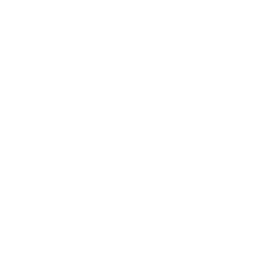
\includegraphics[scale=1]{assets/branding/opa0}
    \vspace{-5.75cm}\\
    {\adjustbox{scale=1.65}{\color{TealDarkCyan}\;V.\;Cryptographic Lattices}}
    \vspace{.25cm}
    \begin{minipage}{.78\textwidth}
      \scriptsize\color{Ink}
      \textbf{Big picture.}\; LWE/LWR are noisy decoding templates; SIS is a short-relation template.\\[.2cm]
      \textbf{Details to watch.}\; $q$-ary lattices, rings, modules, rounding, parameters, and reductions.
    \end{minipage}
    {\ }\vspace{2.1cm}\\
    \bigskip
  \end{center}
\end{frame}

\begin{frame}[shrink=10]{\textbf{V. Cryptographic Lattices}}{$q$-ary Lattices}
\defbox[$q$-ary lattice from a matrix]{
Let $\mat A\in\Z_q^{m\times n}$. Define
\[
  \Lambda_q^\perp(\mat A)
  =\set{x\in\Z^n:\mat A x\equiv 0\pmod q}.
\]
This is an integer lattice containing $q\Z^n$.
}
\begin{itemize}
  \item Modular linear algebra becomes lattice geometry after lifting to $\Z^n$.
  \item The determinant is typically a power of $q$ when $\mat A$ has full rank modulo $q$.
  \item Short integer relations modulo $q$ are short lattice vectors.
\end{itemize}
\textbf{Toy example.}\; Take $q=5$ and $\mat A=[1\ \ 2]$.
Then
\[
  \Lambda_5^\perp(\mat A)=\set{(x_1,x_2)\in\Z^2:x_1+2x_2\equiv0\pmod5}.
\]
The vector $(3,1)$ lies in this lattice because $3+2=5$.
\vspace{-.1cm}
\begin{center}
\begin{tikzpicture}
  \node[process] (mod) {modular equations\\[-1pt]$\mat A x=0\bmod q$};
  \node[process blue, right=1.4cm of mod] (lat) {integer lattice\\[-1pt]$x\in\Lambda_q^\perp(\mat A)$};
  \node[process amber, right=1.4cm of lat] (short) {short relation\\[-1pt]$\norm{x}$ small};
  \draw[flow] (mod) -- (lat);
  \draw[flow blue] (lat) -- (short);
\end{tikzpicture}
\end{center}
\end{frame}

\begin{frame}[shrink=8]{\textbf{V. Cryptographic Lattices}}{Problem Family Map}
\begin{center}
\renewcommand{\arraystretch}{1.22}
\begin{tabular}{p{.19\textwidth}p{.30\textwidth}p{.39\textwidth}}
\toprule
Problem & Public data & Hidden object \\
\midrule
LWE & noisy linear equations over $\Z_q$ & secret $s$ or non-randomness \\
Ring-LWE & noisy equations over $R_q=\Z_q[x]/(f)$ & polynomial secret $s$ \\
Module-LWE & noisy equations over $R_q^k$ & vector of polynomial secrets \\
LWR & rounded linear equations & rounding error replaces sampled noise \\
SIS & matrix $\mat A$ over $\Z_q$ & short relation $x$ with $\mat A x=0$ \\
Module-SIS & matrix over $R_q$ & short module relation \\
\bottomrule
\end{tabular}
\end{center}
\vspace{-.1cm}
\textbf{Two recurring templates.}
\[
  \text{LWE side: noisy or rounded equations}
  \qquad
  \text{SIS side: short modular relations.}
\]
\textbf{Why so many names?}\; Plain matrix problems are conceptually clean.
Ring and module versions add algebraic structure for compact keys and fast arithmetic while trying to preserve lattice hardness.
\end{frame}

\begin{frame}[shrink=6]{\textbf{V. Cryptographic Lattices}}{The Common Hardness Pattern}
\small
\begin{center}
\renewcommand{\arraystretch}{1.20}
\begin{tabular}{>{\bfseries}p{.22\textwidth}p{.31\textwidth}p{.33\textwidth}}
\toprule
Lens & LWE/LWR side & SIS side \\
\midrule
Public object & samples $(\mat A,b)$ & matrix or module map $\mat A$ \\
Hidden witness & secret $s$ and small error & nonzero short relation $x$ \\
Verification & decode or distinguish & check $\mat A x=0\bmod q$ and $\norm{x}\le\beta$ \\
Geometry & BDD / closest point & SVP-like short-vector search \\
Structured forms & rings and modules compress $\mat A$ & rings and modules compress relations \\
\bottomrule
\end{tabular}
\end{center}
\vspace{-.1cm}
\thmbox[One template, many interfaces]{
The details change from vectors to polynomials to modules, but the hard step is always geometric:
recover the small object hidden inside a modular algebraic description.
}
\end{frame}

\begin{frame}[shrink=5]{\textbf{V. Cryptographic Lattices}}{SIS}
\defbox[Short Integer Solution]{
Given a random matrix $\mat A\in\Z_q^{m\times n}$, find a nonzero short vector $x\in\Z^n$ such that
\[
  \mat A x\equiv 0\pmod q.
\]
}
\begin{columns}[T,onlytextwidth]
\begin{column}{.48\textwidth}
\textcolor{TealDarkCyan}{\textbf{Lattice form}}
\[
  x\in\Lambda_q^\perp(\mat A),\qquad 0<\norm{x}\le \beta.
\]
SIS is a short-vector problem in a $q$-ary lattice.
\textbf{Toy relation.}\; For $\mat A=[1\ \ 2]\bmod5$, $x=(3,1)$ satisfies $\mat A x=5\equiv0$.
Real SIS uses dimensions where finding such short relations is hard.
\end{column}
\begin{column}{.48\textwidth}
\textcolor{TealDarkCyan}{\textbf{Cryptographic intuition}}
\begin{itemize}
  \item Easy to verify: compute $\mat A x\bmod q$.
  \item Hard to find when parameters make short relations rare.
  \item Gives collision-resistant hashing and signatures.
\end{itemize}
\end{column}
\end{columns}
\end{frame}

\begin{frame}{\textbf{V. Cryptographic Lattices}}{Visualization: SIS as Congruence Lines}
\small
\begin{columns}[T,onlytextwidth]
\begin{column}{.50\textwidth}
\textbf{Toy kernel.}\; For $q=5$ and $\mat A=[1\ \ 2]$,
\[
  x_1+2x_2\equiv0\pmod5.
\]
The lattice is the union of integer points on the parallel lines
\[
  x_1+2x_2=5k,\qquad k\in\Z.
\]
\textbf{SIS asks for a short nonzero point on these lines.}
\end{column}
\begin{column}{.46\textwidth}
\begin{center}
\begin{tikzpicture}[scale=.43,transform shape]
  \useasboundingbox (-5.3,-5.55) rectangle (5.3,4.4);
  \draw[panel] (-5.3,-4.4) rectangle (5.3,4.4);
  \begin{scope}
  \clip (-5.3,-4.4) rectangle (5.3,4.4);
  \foreach \x in {-5,...,5}{
    \draw[thin lattice line] (\x,-4.1) -- (\x,4.1);
  }
  \foreach \y in {-4,...,4}{
    \draw[thin lattice line] (-5.1,\y) -- (5.1,\y);
  }
  \foreach \k in {-2,...,2}{
    \draw[BlueCode!32,line width=.9pt] (-5,{(5*\k+5)/2}) -- (5,{(5*\k-5)/2});
  }
  \foreach \x in {-5,...,5}{
    \foreach \y in {-4,...,4}{
      \node[circle,fill=Ink!35,inner sep=.8pt] at (\x,\y) {};
    }
  }
  \foreach \x/\y in {0/0,3/1,1/2,-2/1,-4/2,2/-1,4/-2,-1/-2,-3/-1}{
    \node[circle,fill=ErrorRed,inner sep=2.0pt] at (\x,\y) {};
  }
  \draw[short vector] (0,0) -- (3,1) node[above right] {$(3,1)$};
  \end{scope}
  \node[caption text,align=center,text width=5.5cm] at (0,-5.05)
    {red points satisfy $x_1+2x_2\equiv0\bmod 5$};
\end{tikzpicture}
\end{center}
\end{column}
\end{columns}
\end{frame}

\begin{frame}[shrink=8]{\textbf{V. Cryptographic Lattices}}{LWE}
\defbox[Learning With Errors]{
Let $s\in\Z_q^n$ be secret. Given samples
\[
  (a_i,\ b_i=\inner{a_i}{s}+e_i \bmod q),
\]
where $a_i\leftarrow\Z_q^n$ and $e_i$ is small, recover $s$ or distinguish the samples from uniform.
}
\begin{itemize}
  \item Without error, this is linear algebra over $\Z_q$.
  \item With small error, the equations are only approximately consistent.
  \item The error hides the exact lattice hyperplanes that would reveal $s$.
\end{itemize}
\bigskip
\textbf{\color{red}Core idea.}\; Noise turns an easy algebra problem into a closest-vector style problem.
\textbf{One sample.}\; Let $q=17$, $a=(3,5)$, $s=(4,2)$, and $e=-1$.
Then
\[
  b=\inner{a}{s}+e=3\cdot4+5\cdot2-1=21\equiv4\pmod{17}.
\]
Without the error, the value would be $5$; the small shift hides the exact equation.
\end{frame}

\begin{frame}{\textbf{V. Cryptographic Lattices}}{Visualization: LWE Thickens Exact Equations}
\small
\begin{columns}[T,onlytextwidth]
\begin{column}{.46\textwidth}
\textbf{No error.}\; Each equation cuts the secret space by a thin modular hyperplane.

\medskip
\textbf{With error.}\; The hyperplane becomes a strip:
\[
  \inner{a_i}{s}\approx b_i\pmod q.
\]
\textbf{Many strips intersect near the secret, but the exact intersection is blurred.}
\end{column}
\begin{column}{.50\textwidth}
\begin{center}
\begin{tikzpicture}[scale=.72]
  \useasboundingbox (-3.3,-3.2) rectangle (3.3,2.6);
  \draw[panel] (-3.25,-2.55) rectangle (3.25,2.55);
  \begin{scope}
    \clip (-3.25,-2.55) rectangle (3.25,2.55);
    \begin{scope}[rotate=22]
      \foreach \k in {-3,...,3}{
        \fill[AmberCode!10] (-4,{.72*\k-.12}) rectangle (4,{.72*\k+.12});
        \draw[BlueCode!38,line width=.65pt] (-4,{.72*\k}) -- (4,{.72*\k});
      }
    \end{scope}
    \begin{scope}[rotate=-38]
      \foreach \k in {-3,...,3}{
        \fill[TealDarkCyan!8] (-4,{.78*\k-.10}) rectangle (4,{.78*\k+.10});
        \draw[TealDarkCyan!38,line width=.65pt] (-4,{.78*\k}) -- (4,{.78*\k});
      }
    \end{scope}
  \end{scope}
  \node[circle,fill=ErrorRed,inner sep=2.4pt,label={[tiny label]above:$s$}] at (.35,.25) {};
  \draw[ErrorRed!60,fill=ErrorRed!8] (.35,.25) circle (.38);
  \node[caption text,align=center] at (0,-3.02)
    {error turns exact hyperplanes into noisy strips};
\end{tikzpicture}
\end{center}
\end{column}
\end{columns}
\end{frame}

\begin{frame}[shrink=8]{\textbf{V. Cryptographic Lattices}}{LWE as Bounded Distance Decoding}
Collect $m$ samples into a matrix $\mat A\in\Z_q^{m\times n}$ and vector
\[
  b=\mat A s+e\pmod q.
\]
\defbox[Decoding view]{
The vector $b$ is close to the code/lattice generated by columns of $\mat A$ modulo $q$. Recovering $s$ means identifying the nearby structured point despite the error $e$.
}
\textbf{Decoding analogy.}\; In the toy sample above, $4$ is close to the noiseless value $5$ modulo $17$.
BDD asks for the hidden structured point when many coordinates have small errors.
\begin{center}
\begin{tikzpicture}[scale=.82]
  \node[process] (secret) {$s$};
  \node[process blue, right=1.0cm of secret] (linear) {$\mat A s$};
  \node[process amber, right=1.0cm of linear] (noise) {$\mat A s+e$};
  \node[process red, right=1.0cm of noise] (public) {$b\bmod q$};
  \draw[flow] (secret) -- node[above,tiny label] {linear map} (linear);
  \draw[flow blue] (linear) -- node[above,tiny label] {small error} (noise);
  \draw[flow amber] (noise) -- node[above,tiny label] {reduce mod $q$} (public);
\end{tikzpicture}
\end{center}
\end{frame}

\begin{frame}{\textbf{V. Cryptographic Lattices}}{Penetrating Example: Primal LWE Attack I}
\small
\defbox[LWE as BDD]{
Given $\mat A\in\Z_q^{m\times n}$ and $b=\mat A s+e\pmod q$, define the $q$-ary lattice
\[
  \Lambda_q(\mat A)=\set{\mat A z+q y:z\in\Z^n,\ y\in\Z^m}\subseteq\Z^m.
\]
Then $\mat A s\in\Lambda_q(\mat A)$ and $b$ is close to it by the error vector $e$.
}
\textbf{Attack question.}\; The attacker sees $\mat A$ and $b$, but not $s$ or $e$:
\[
  \text{find the closest point of }\Lambda_q(\mat A)\text{ to }b.
\]
Once that point is recovered as $\mat A s$, solving for $s$ is linear algebra modulo $q$.

\textbf{Why this is penetrating.}\; LWE is not just ``linear equations with noise.''  It is a decoding problem in a high-dimensional modular lattice where the noise radius is deliberately below the expected lattice spacing.
\end{frame}

\begin{frame}{\textbf{V. Cryptographic Lattices}}{Penetrating Example: Primal LWE Attack II}
\small
\begin{columns}[T,onlytextwidth]
\begin{column}{.49\textwidth}
\textbf{Concrete sample.}\; Let $q=17$,
\[
  \mat A=\begin{bmatrix}3&5\\7&4\\2&9\end{bmatrix},\qquad
  s=\begin{bmatrix}4\\2\end{bmatrix},\qquad
  e=\begin{bmatrix}1\\-1\\0\end{bmatrix}.
\]
Then
\[
  \mat A s\equiv (5,2,9),\qquad b=(6,1,9)\pmod{17}.
\]
\end{column}
\begin{column}{.47\textwidth}
\textbf{Geometric meaning.}
\[
  b-(\mat A s)=e,\qquad \norm{e}=\sqrt2.
\]
The public vector $b$ is a point near the hidden lattice point $\mat A s$.
The error vector is the displacement that hides the exact equation.
\end{column}
\end{columns}
\begin{center}
\begin{tikzpicture}[scale=.78]
  \foreach \i in {-2,...,2}{
    \foreach \j in {-2,...,2}{
      \coordinate (p) at ({\i+.55*\j},{.62*\j});
      \node[lattice point] at (p) {};
    }
  }
  \coordinate (as) at (.55,.62);
  \coordinate (bb) at (.88,.34);
  \draw[ErrorRed!35,fill=ErrorRed!8] (as) circle (.48);
  \node[circle,fill=BlueCode,inner sep=2pt,label={[tiny label]above:$\mat A s$}] at (as) {};
  \node[circle,fill=ErrorRed,inner sep=2pt,label={[tiny label]right:$b$}] at (bb) {};
  \draw[flow red] (as) -- node[midway,below,tiny label] {$e$} (bb);
  \node[caption text,fill=white,inner sep=1pt,align=center] at (0,-1.24)
    {LWE attack surface: BDD in a $q$-ary lattice};
\end{tikzpicture}
\end{center}
\end{frame}

\begin{frame}[shrink=8]{\textbf{V. Cryptographic Lattices}}{Structured Algebra: Rings and Modules}
\defbox[Ring used in structured lattice cryptography]{
Let
\[
  R=\Z[x]/(f(x)),\qquad R_q=R/qR.
\]
An element of $R_q$ is a polynomial with coefficients modulo $q$, reduced by the rule $f(x)=0$.
}
\begin{columns}[T,onlytextwidth]
\begin{column}{.48\textwidth}
\textcolor{TealDarkCyan}{\textbf{Ring viewpoint}}
\begin{itemize}
  \item One ring element stores many coefficients.
  \item Multiplication by $a\in R_q$ is a structured linear map.
  \item Ring-LWE is LWE with this special structure.
\end{itemize}
\end{column}
\begin{column}{.48\textwidth}
\textcolor{TealDarkCyan}{\textbf{Module viewpoint}}
\begin{itemize}
  \item A module vector lies in $R_q^k$.
  \item Module rank $k$ tunes the amount of structure.
  \item Module-LWE sits between plain LWE and Ring-LWE.
\end{itemize}
\end{column}
\end{columns}
\textbf{Concrete reading.}\; If each polynomial has degree $d-1$, then one module vector in $R_q^k$ contains $kd$ ordinary modular coefficients.
\end{frame}

\begin{frame}{\textbf{V. Cryptographic Lattices}}{Visualization: Ring Multiplication Is Structured Linear Algebra}
\small
\begin{columns}[T,onlytextwidth]
\begin{column}{.48\textwidth}
\[
  a(x)s(x)\bmod f(x),q
\]
is polynomial multiplication, but after expanding coefficients it becomes
\[
  \mat M_a\,\vect s \bmod q.
\]
\textbf{The matrix $\mat M_a$ is not arbitrary.}\; Its rows are shifted and signed versions of the coefficients of $a$.
\end{column}
\begin{column}{.48\textwidth}
\begin{center}
\[
\mat M_a=
\begin{bmatrix}
 a_0 & -a_3 & -a_2 & -a_1\\
 a_1 &  a_0 & -a_3 & -a_2\\
 a_2 &  a_1 &  a_0 & -a_3\\
 a_3 &  a_2 &  a_1 &  a_0
\end{bmatrix}
\]
\vspace{-.15cm}
{\sffamily\small\color{Ink!72} example shape for $f(x)=x^4+1$}
\end{center}
\end{column}
\end{columns}
\vfill
\textbf{Security tension.}\; Structure makes schemes smaller and faster, but attackers may also try to exploit it.
\end{frame}

\begin{frame}[shrink=7]{\textbf{V. Cryptographic Lattices}}{Ring-LWE}
\defbox[Ring Learning With Errors]{
Choose a secret $s\in R_q$. Given samples
\[
  (a_i,\ b_i=a_i s+e_i \bmod q),
\]
where $a_i\leftarrow R_q$ and $e_i$ is a small polynomial, recover $s$ or distinguish the samples from uniform over $R_q^2$.
}
\begin{itemize}
  \item It is the LWE template, but scalars are polynomial ring elements.
  \item Coefficient expansion turns it into ordinary LWE with highly structured matrices.
  \item The noise is small in the coefficient embedding used by the scheme.
\end{itemize}
\textbf{Toy shape.}\; In $R_q=\Z_q[x]/(x^4+1)$, a secret has the form
\[
  s=s_0+s_1x+s_2x^2+s_3x^3.
\]
One sample hides all four coefficients at once through polynomial multiplication plus error.
\end{frame}

\begin{frame}[shrink=7]{\textbf{V. Cryptographic Lattices}}{Module-LWE}
\defbox[Module Learning With Errors]{
Let $\mat A\in R_q^{m\times k}$, $s\in R_q^k$, and let $e\in R^m$ be small. The public vector is
\[
  b=\mat A s+e\pmod q.
\]
The problem is to recover $s$ or distinguish $(\mat A,b)$ from uniform.
}
\begin{columns}[T,onlytextwidth]
\begin{column}{.48\textwidth}
\textcolor{TealDarkCyan}{\textbf{Interpolation}}
\begin{itemize}
  \item Degree $d=1$ gives ordinary matrix LWE.
  \item Rank $k=1$ resembles the ring setting.
  \item Larger $k$ reduces reliance on one ring equation.
\end{itemize}
\end{column}
\begin{column}{.48\textwidth}
\textcolor{TealDarkCyan}{\textbf{Why cryptographers use it}}
\begin{itemize}
  \item Compact public keys.
  \item Fast number-theoretic transforms.
  \item Adjustable tradeoff between structure and size.
\end{itemize}
\end{column}
\end{columns}
\textbf{Mental model.}\; Module-LWE is a block lattice problem: every entry is a polynomial block, and the whole object expands to a larger ordinary lattice instance.
\end{frame}

\begin{frame}[shrink=8]{\textbf{V. Cryptographic Lattices}}{LWR}
\defbox[Learning With Rounding]{
Let $p<q$ and let $\operatorname{Round}_{q\to p}:\Z_q\to\Z_p$ keep only a coarse approximation to a residue modulo $q$.
Samples have the form
\[
  (a_i,\ b_i=\operatorname{Round}_{q\to p}(\inner{a_i}{s})).
\]
}
\begin{itemize}
  \item LWE adds explicit random error:
  \[
    b_i=\inner{a_i}{s}+e_i\bmod q.
  \]
  \item LWR replaces explicit error by deterministic quantization error.
  \item The hidden error is bounded by the rounding interval.
\end{itemize}
\textbf{Concrete rounding picture.}\; Mapping $\Z_{17}$ to $\Z_4$ groups several residues together.
Knowing only the rounded bin hides the exact value of $\inner{a_i}{s}$.
\end{frame}

\begin{frame}{\textbf{V. Cryptographic Lattices}}{Visualization: LWR as Quantization}
\small
\begin{center}
\begin{tikzpicture}[x=.58cm,y=1cm]
  \draw[->,line width=.9pt,draw=Ink!65] (-.2,0) -- (17.6,0) node[right] {$\Z_{17}$};
  \foreach \x in {0,...,17}{
    \draw[Ink!35] (\x,-.10) -- (\x,.10);
  }
  \foreach \a/\b/\lab/\col in {0/4/0/BlueCode,4/8/1/TealDarkCyan,8/13/2/AmberCode,13/17/3/ErrorRed}{
    \fill[\col!11] (\a,-.32) rectangle (\b,.32);
    \draw[\col!70,line width=.8pt] (\a,-.32) rectangle (\b,.32);
    \node[tiny label,\col!80!black] at ({(\a+\b)/2},.65) {$\lab$};
  }
  \node[circle,fill=BlueCode,inner sep=2.1pt] at (5,0) {};
  \node[circle,fill=ErrorRed,inner sep=2.1pt] at (6,0) {};
  \node[tiny label,BlueCode!80!black,align=center] at (3.55,-.82) {noiseless\\value};
  \node[tiny label,ErrorRed!85!black,align=center] at (8.10,-.82) {nearby\\value};
  \draw[BlueCode!65,line width=.6pt] (4.12,-.55) -- (4.92,-.08);
  \draw[ErrorRed!65,line width=.6pt] (7.42,-.55) -- (6.08,-.08);
  \draw[<->,ErrorRed!70,line width=.8pt] (4,-1.16) -- (8,-1.16);
  \node[tiny label,ErrorRed!85!black] at (6,-1.46) {same rounded output};
\end{tikzpicture}
\end{center}
\vspace{-.1cm}
\textbf{Meaning.}\; Rounding discards low-order information. The lost information behaves like a controlled error term in a decoding problem.
\end{frame}

\begin{frame}[shrink=8]{\textbf{V. Cryptographic Lattices}}{Module-SIS}
\defbox[Module Short Integer Solution]{
Given $\mat A\in R_q^{\ell\times k}$, find a nonzero short vector
\[
  x\in R^k
\]
such that
\[
  \mat A x\equiv 0\pmod q.
\]
}
\begin{columns}[T,onlytextwidth]
\begin{column}{.48\textwidth}
\textcolor{TealDarkCyan}{\textbf{Relation to SIS}}
\begin{itemize}
  \item SIS uses integer vectors over $\Z_q$.
  \item Module-SIS uses polynomial vectors over $R_q$.
  \item Ring-SIS is the rank-one structured case.
\end{itemize}
\end{column}
\begin{column}{.48\textwidth}
\textcolor{TealDarkCyan}{\textbf{Cryptographic role}}
\begin{itemize}
  \item Short relations are easy to verify.
  \item They are hard to find at secure dimensions.
  \item This supports hash, commitment, and signature-style constructions.
\end{itemize}
\end{column}
\end{columns}
\textbf{Mental model.}\; Module-SIS asks for a short polynomial-vector collision in a public modular linear map.
\end{frame}

\begin{frame}{\textbf{V. Cryptographic Lattices}}{How the Named Problems Fit Together}
\small
\begin{center}
\begin{tikzpicture}[node distance=.58cm,scale=.84,transform shape]
  \node[process] (plain) {plain matrix\\over $\Z_q$};
  \node[process blue,below left=of plain,xshift=-.3cm] (lwe) {LWE\\noise};
  \node[process amber,below right=of plain,xshift=.3cm] (sis) {SIS\\short relation};
  \node[process blue,below=of lwe] (rlwe) {Ring/Module-LWE\\polynomial blocks};
  \node[process amber,below=of sis] (msis) {Ring/Module-SIS\\polynomial blocks};
  \node[process red,below=of rlwe] (lwr) {LWR/Module-LWR\\rounding};
  \draw[flow] (plain) -- (lwe);
  \draw[flow amber] (plain) -- (sis);
  \draw[flow blue] (lwe) -- (rlwe);
  \draw[flow amber] (sis) -- (msis);
  \draw[flow red] (rlwe) -- (lwr);
\end{tikzpicture}
\end{center}
\begin{columns}[T,onlytextwidth]
\begin{column}{.48\textwidth}
\textbf{LWE side.}\; Noise or rounding turns exact modular equations into bounded-distance decoding.
\end{column}
\begin{column}{.48\textwidth}
\textbf{SIS side.}\; Shortness turns a modular kernel into a short-vector search problem.
\end{column}
\end{columns}
\end{frame}

\begin{frame}[shrink=8]{\textbf{V. Cryptographic Lattices}}{Trapdoors}
\defbox[Lattice trapdoor, informal]{
A public basis may be bad for solving CVP or sampling short vectors, while a secret basis of the same lattice is good.
}
\begin{columns}[T,onlytextwidth]
\begin{column}{.48\textwidth}
\textcolor{TealDarkCyan}{\textbf{Public view}}
\begin{itemize}
  \item Random-looking modular matrix.
  \item Hard basis for the associated lattice.
  \item Short preimages look difficult to find.
\end{itemize}
\end{column}
\begin{column}{.48\textwidth}
\textcolor{TealDarkCyan}{\textbf{Secret view}}
\begin{itemize}
  \item Structured short basis.
  \item Efficient Gaussian sampling.
  \item Enables signatures and identity-based encryption.
\end{itemize}
\end{column}
\end{columns}
\bigskip
\thmbox[Security shape]{
The public key describes the lattice; the trapdoor describes it well.
}
\textbf{Example shape.}\; The public matrix may define the same lattice as a secret short basis.
To outsiders it resembles a bad basis; to the owner it resembles a basis exposing short vectors.
\end{frame}

\begin{frame}{\textbf{V. Cryptographic Lattices}}{Visualization: Public Basis, Secret Basis}
\small
\begin{center}
\begin{tikzpicture}[scale=.66]
  \begin{scope}[shift={(-3.55,0)}]
    \foreach \i in {-3,...,3}{
      \foreach \j in {-3,...,3}{
        \node[lattice point] at ({\i+.35*\j},{.78*\j}) {};
      }
    }
    \draw[basis vector] (0,0) -- (2.75,.78) node[above] {$p_1$};
    \draw[basis vector] (0,0) -- (2.40,0) node[below] {$p_2$};
    \node[caption text,align=center] at (0,-2.35)
      {public description\\long, skew, attack-resistant};
  \end{scope}
  \begin{scope}[shift={(3.55,0)}]
    \foreach \i in {-3,...,3}{
      \foreach \j in {-3,...,3}{
        \node[lattice point] at ({\i+.35*\j},{.78*\j}) {};
      }
    }
    \draw[short vector] (0,0) -- (1,0) node[below] {$s_1$};
    \draw[short vector] (0,0) -- (.35,.78) node[left] {$s_2$};
    \node[caption text,align=center] at (0,-2.35)
      {secret trapdoor\\short, stable, sampleable};
  \end{scope}
  \node[process amber] at (0,2.25) {same lattice point set};
\end{tikzpicture}
\end{center}
\textbf{Meaning.}\; A trapdoor is not a different lattice; it is a better hidden coordinate system for the same public lattice.
\end{frame}

\begin{frame}[shrink=6]{\textbf{V. Cryptographic Lattices}}{Worst-case to Average-case}
\thmbox[Ajtai-Regev philosophy]{
Solving certain random lattice problems on average would imply algorithms for hard lattice problems in the worst case.
}
\begin{itemize}
  \item SIS is connected to worst-case SIVP and related short-vector problems.
  \item LWE is connected to worst-case GapSVP and SIVP under suitable parameters.
  \item Ring and module variants use structured ideal or module lattice assumptions.
  \item This is stronger evidence than a purely ad hoc average-case assumption.
\end{itemize}
\textbf{Concrete reading.}\; A solver for random-looking LWE samples would become a solver for geometric problems on arbitrary lattices; structured variants trade some generality for efficiency.
\vspace{-.1cm}
\begin{center}
\begin{tikzpicture}[node distance=.8cm]
  \node[process] (worst) {worst-case\\{}lattices};
  \node[process blue, right=1.3cm of worst] (reduce) {reduction};
  \node[process amber, right=1.3cm of reduce] (avg) {random\\instances};
  \node[process red, right=1.3cm of avg] (crypto) {public-key\\crypto};
  \draw[flow] (worst) -- (reduce);
  \draw[flow blue] (reduce) -- (avg);
  \draw[flow amber] (avg) -- (crypto);
\end{tikzpicture}
\end{center}
\end{frame}

\begin{frame}{\textbf{V. Cryptographic Lattices}}{What Parameters Control}
\scriptsize
\begin{center}
\renewcommand{\arraystretch}{1.12}
\begin{tabular}{>{\bfseries}p{.22\textwidth}p{.66\textwidth}}
\toprule
Parameter & Role \\
\midrule
$n$ & Main security dimension. \\
$q$ & Modulus and wraparound scale. \\
$m$ & Number of samples or equations. \\
$d$ & Ring degree; coefficients per polynomial. \\
$k$ & Module rank; amount of structure. \\
$p$ & LWR rounded output modulus. \\
$\alpha q$ & LWE error scale. \\
$\beta$ & SIS shortness bound. \\
\bottomrule
\end{tabular}
\end{center}
\vspace{-.1cm}
\textbf{\color{red}Design tension.}\; Correctness wants small noise and short vectors; security wants them not too small.
\end{frame}

\begin{frame}{\textbf{V. Cryptographic Lattices}}{Visualization: Parameter Tradeoff}
\small
\begin{center}
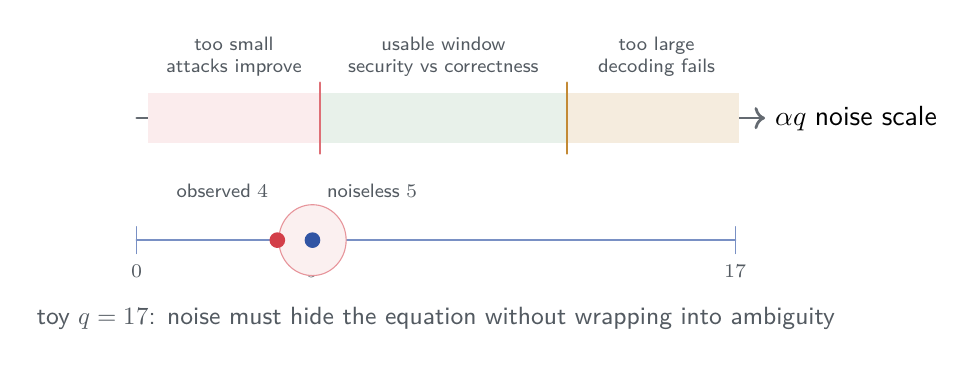
\begin{tikzpicture}[x=.95cm,y=1cm]
  \draw[->,line width=1pt,draw=Ink!65] (0,0) -- (8.4,0) node[right] {$\alpha q$ noise scale};
  \fill[ErrorRed!10] (.15,-.32) rectangle (2.45,.32);
  \fill[GoodGreen!12] (2.45,-.32) rectangle (5.75,.32);
  \fill[AmberCode!14] (5.75,-.32) rectangle (8.05,.32);
  \draw[ErrorRed!75,line width=.9pt] (2.45,-.45) -- (2.45,.45);
  \draw[AmberCode!85,line width=.9pt] (5.75,-.45) -- (5.75,.45);
  \node[tiny label,align=center] at (1.30,.78) {too small\\attacks improve};
  \node[tiny label,align=center] at (4.10,.78) {usable window\\security vs correctness};
  \node[tiny label,align=center] at (6.95,.78) {too large\\decoding fails};

  \draw[BlueCode!65,line width=.9pt] (0,-1.55) -- (8,-1.55);
  \foreach \x/\lab in {0/0,2.35/5,8/17}{
    \draw[BlueCode!65] (\x,-1.72) -- (\x,-1.38);
    \node[tiny label] at (\x,-1.95) {$\lab$};
  }
  \draw[ErrorRed!55,fill=ErrorRed!8] (2.35,-1.55) circle (.45);
  \node[circle,fill=BlueCode,inner sep=2pt] at (2.35,-1.55) {};
  \node[circle,fill=ErrorRed,inner sep=2pt] at (1.88,-1.55) {};
  \node[tiny label,align=center] at (3.15,-.92) {noiseless $5$};
  \node[tiny label,align=center] at (1.15,-.92) {observed $4$};
  \node[caption text] at (4,-2.55)
    {toy $q=17$: noise must hide the equation without wrapping into ambiguity};
\end{tikzpicture}
\end{center}
\end{frame}

\begin{frame}[shrink=6]{\textbf{V. Cryptographic Lattices}}{Summary}
\begin{itemize}
  \item A lattice is a discrete additive subgroup of Euclidean space.
  \item Bases are algebraic descriptions; lengths and volumes are geometric invariants.
  \item Minkowski's theorem proves short vectors exist, but does not find them efficiently.
  \item SVP, CVP, SIVP, and GapSVP formalize the hard search and decision tasks.
  \item SIS and Module-SIS ask for short modular relations.
  \item LWE, Ring-LWE, Module-LWE, and LWR ask attackers to solve noisy or rounded modular equations.
\end{itemize}
\bigskip
\thmbox[One-line takeaway]{
Lattice cryptography is built on the gap between compact algebraic descriptions and difficult Euclidean search.
}
\textbf{Examples to remember.}\; Minkowski: area $>4$ forces an integer point in $\Z^2$.
LLL: $(1001,1000)-(1000,999)=(1,1)$ exposes hidden shortness.
LWE/LWR: exact linear algebra becomes noisy or rounded decoding.
\end{frame}


%-------------------------------------------------------
% CLOSING FRAME
%-------------------------------------------------------
\HardProblemLens{Remember the two templates: noisy decoding for LWE/LWR and short relations for SIS.}
\begin{frame}[plain]
  \begin{center}\bfseries\centering
    \vspace{1.35cm}
    {\Huge\color{TealDarkCyan} Thank You}\\[.5cm]
    {\large\color{black} Ji, Yong-hyeon}\\[.3cm]
    {\normalsize\texttt{hacker3740@gmail.com}}\\[.5cm]
    \begin{minipage}{.76\textwidth}
      \small\color{Ink}
      \textbf{Big picture.}\; Lattice cryptography is built from compact public algebra and hard hidden geometry.\\[.2cm]
      \textbf{Details to remember.}\; LWE/LWR are noisy or rounded decoding; SIS and Module-SIS are short-relation search.
    \end{minipage}\\[.5cm]
    {\small\color{gray} Enjoying Math $\cdot$ Hard Problems $\cdot$ 2026}
    \bigskip
  \end{center}
\end{frame}

\end{document}
